%% =========================================================================
%% Delegation cascades: stable stationary computation in an evolutionary game
%% with strategic chain depth
%%
%% Prepared for Applied Mathematics and Computation (Elsevier).
%% Elsevier CAS bundle, single-column layout (cas-sc.cls).
%%
%%   pdflatex main && bibtex main && pdflatex main && pdflatex main
%% =========================================================================

%% Loading float ahead of the class stops the algorithm package from
%% re-registering the float counters, which otherwise emits one
%% "destination with the same identifier" warning per float.
\RequirePackage{float}
\documentclass[a4paper,fleqn]{cas-sc}

\usepackage[numbers,sort&compress]{natbib}

%% cas-sc leaves \sfdefault at the EC family, whose \textsf is embedded as a
%% Type 3 PK bitmap; the strategy labels use \textsf on nearly every page.
\renewcommand{\sfdefault}{lmss}
\renewcommand{\ttdefault}{lmtt}

\usepackage{placeins}
\usepackage{algorithm}
\usepackage{algpseudocode}
\usepackage{tikz}
\usetikzlibrary{arrows.meta,positioning,calc}

\newtheorem{theorem}{Theorem}
\newtheorem{proposition}[theorem]{Proposition}
\newtheorem{lemma}[theorem]{Lemma}
\newtheorem{corollary}[theorem]{Corollary}
\newdefinition{remark}[theorem]{Remark}
\newproof{pf}{Proof}

\definecolor{cAS}{HTML}{0072B2}
\definecolor{cCS}{HTML}{009E73}
\definecolor{cCAS}{HTML}{E69F00}
\definecolor{cAU}{HTML}{D55E00}
\definecolor{cGrey}{HTML}{4D4D4D}

\newcommand{\AS}{\textsf{AS}}
\newcommand{\CS}{\textsf{CS}}
\newcommand{\CAS}{\textsf{CAS}}
\newcommand{\AU}{\textsf{AU}}
\newcommand{\piP}{\pi_{P}}
\newcommand{\piS}{\pi_{S}}

%% Full-width floats in a single-column layout fill most of a top area, so the
%% class defaults leave a backlog that never clears and every figure prints two
%% or three pages after the text that discusses it.
\renewcommand{\topfraction}{0.9}
\renewcommand{\bottomfraction}{0.8}
\renewcommand{\textfraction}{0.07}
\renewcommand{\floatpagefraction}{0.75}

\begin{document}
\let\WriteBookmarks\relax
\def\floatpagepagefraction{1}
\def\textpagefraction{.001}

\shorttitle{Delegation cascades: stable stationary computation}
\shortauthors{T.-K. Huynh et al.}

\title[mode=title]{Delegation cascades: stable stationary computation in an
evolutionary game with strategic chain depth}

% =========================================================================
% All three authors contributed equally; the shared first authorship is
% carried by the \fnmark[1]/\fntext[1] note below. Applied Mathematics and
% Computation does not allow authorship changes after acceptance.
% =========================================================================

\author[1,2]{Trung-Kiet Huynh}[orcid=0009-0000-5463-754X]
\cormark[1]
\fnmark[1]
\ead{23122039@student.hcmus.edu.vn}
\credit{Conceptualization, Methodology, Software, Formal analysis,
Investigation, Validation, Visualization, Writing -- original draft,
Writing -- review \& editing}

\author[1,2]{Dao Sy Duy Minh}[orcid=0009-0002-4501-2788]
\fnmark[1]
\ead{23122041@student.hcmus.edu.vn}
\credit{Conceptualization, Methodology, Software, Formal analysis,
Investigation, Validation, Visualization, Writing -- original draft,
Writing -- review \& editing}

\author[1,2]{Chi-Nguyen Tran}[orcid=0009-0007-6716-7269]
\fnmark[1]
\ead{23122044@student.hcmus.edu.vn}
\credit{Conceptualization, Methodology, Software, Formal analysis,
Investigation, Validation, Visualization, Writing -- original draft,
Writing -- review \& editing}

\author[1,2]{Nguyen Lam Phu Quy}[orcid=0009-0002-9694-8105]
\ead{23122048@student.hcmus.edu.vn}
\credit{Software, Formal analysis, Investigation, Validation,
Writing -- review \& editing}

\author[1,2]{Pham Phu Hoa}[orcid=0009-0001-5471-2578]
\ead{23122030@student.hcmus.edu.vn}
\credit{Software, Formal analysis, Investigation, Validation,
Writing -- review \& editing}

\affiliation[1]{organization={Faculty of Information Technology,
            University of Science (HCMUS)},
            city={Ho Chi Minh City},
            country={Vietnam}}

\affiliation[2]{organization={Vietnam National University -- Ho Chi
            Minh City (VNU-HCM)},
            city={Ho Chi Minh City},
            country={Vietnam}}

\cortext[1]{Corresponding author}
\fntext[1]{These authors contributed equally to this work.}

\begin{abstract}
Software increasingly acts through chains: a principal instructs an agent,
which instructs further agents; each hand-off restates the specification
imperfectly and traces responsibility back only in part. Making delegation
depth a strategic variable in an evolutionary game puts the mutation--selection
chain over population states, $3.0\times10^{27}$ of them, out of reach. We
give a scheme that avoids it. The interaction tensor is summed exactly over the
horizon law; the process is reduced to an embedded chain on the pure designs,
exact as the mutation rate vanishes, with its residual measured against the
full chain; and the fixation probabilities that chain needs follow from a
closed form in $O(Z)$ operations, with the largest exponent factored out of a
sum whose terms otherwise overflow double precision. What the reduction needs
of that evaluation is positivity, but positivity alone does not determine
stationary mass in a nearly decomposable chain. We verify the stationary vector
against an arbitrary-precision reference. Two structural results are analytical.
Realised harm saturates in the depth while
attributed harm carries one extra factor per layer, so for every attribution
retention below one there is a depth beyond which each further hand-off
strictly lowers the principal's bill and never lowers the harm it causes; and
an eventually binding constant attribution floor closes that shelter beyond its
binding depth. Numerically, from a calibration whose depth-zero unsafe frequency
is $0.000$, each loss alone leaves it at or below $0.018$ while the two
together raise it to $0.322$, and a statutory floor under attributed
responsibility reproduces a depth cap's frontier wherever it can reach.
\end{abstract}

\begin{highlights}
\item Delegation depth becomes a strategic variable in an evolutionary race game
\item Realised harm saturates in depth while attributed harm decays
      geometrically
\item A stable $O(Z)$ scheme replaces a chain with $3\times10^{27}$ population
      states
\item Transmission and attribution losses interact: together they reach $0.32$
      unsafe
\item A binding attribution floor closely matches a depth-cap frontier
\end{highlights}

\begin{keywords}
Evolutionary game theory \sep Markov chains \sep Fixation probability \sep
Delegation \sep Liability \sep Multi-agent systems
\MSC[2020]{91A22, 60J10, 65C40, 91A80}
\end{keywords}

\maketitle
%% The author footnote raised by \fnmark[1] is number 1 in the same
%% first-page note block as any \footnote from the body, so the body has
%% to start at 2 or two different notes both come out marked 1.
\setcounter{footnote}{1}

% ===========================================================================
\section{Introduction}
\label{sec:intro}

Software that acts on behalf of someone else is increasingly built as a chain.
A principal issues a specification, an agent decomposes it and instructs
sub-agents, and the sub-agents call further tools and agents. The process that
finally takes an action is then several hand-offs away from the party that
wanted it taken~\citep{wu2023autogen,fourney2024magentic}. Governance of such
systems is written almost entirely at the two ends of the chain: safety
training and evaluation act on the model, and liability, procurement rules and
disclosure requirements act on the
principal~\citep{shavit2023practices,chan2024visibility}. The hand-offs in
between are treated as plumbing.\footnote{We call the result a delegation
cascade. The term denotes compounding per-hand-off loss along a single chain
from a principal to the party that acts, and not the informational cascade
of~\citet{bikhchandani1992theory}, in which independent decision makers
rationally discard their own signals after observing what their predecessors
did.}

A hand-off does two things a model can represent. It transmits a specification
imperfectly, because each layer restates the task in its own terms and the part
most easily dropped is a qualifying clause rather than the task itself.
Degradation under repeated re-encoding is a robust property of transmission
chains: in human cultural transmission the distinctions that nothing selects
for are the first to be lost~\citep{kirby2008cumulative}, and the same decay
appears in recursive machine
generation~\citep{shumailov2024collapse,alemohammad2023mad} and in chains of
language models that each restate what the previous one
wrote~\citep{perez2025telephone,acerbi2023transmission}. It has been measured
on instructions directly: across fourteen frontier models, adherence to
explicitly stated instructions falls with every additional turn, from $0.88$ to
$0.71$ over three turns for the strongest of them~\citep{he2024multiif}.
Failure data from deployed agent frameworks show both effects in the field.
Across annotated traces from seven agent frameworks, the largest single failure
class is rooted in the specification and design of the system itself and the
second in misalignment between agents~\citep{cemri2025mast}; and when faulty
agents are injected deliberately, a linear chain of hand-offs degrades more
than any other topology tested, by $23.7\%$ against $5.5\%$ for a hierarchical
arrangement~\citep{huang2025resilience}. A hand-off also attenuates
responsibility, because harm that reaches the world through several
intermediaries is traced back to the party at the top only in part. The gap
this opens has been named for the case of a machine whose behaviour its
operator cannot predict~\citep{matthias2004gap}; ours is a different source of
the same gap, structural rather than epistemic, and one a principal can widen
at will by adding a layer. Both effects are per-layer, so both compound
geometrically in the number of hand-offs, and a cost that compounds that way is
the classical reason a long hierarchy is expected not to survive
competition~\citep{mcafee1995diseconomies}.

The two effects push a principal in opposite directions. Imperfect transmission
is a private cost, so a principal who is held responsible for what its chain
does has every reason to keep the chain short. Imperfect attribution is a
private benefit, since depth buys a discount on the bill. Which force wins is
not a matter of taste, and neither is the policy question that follows:
whether an instrument that improves transmission, one that restores
attribution, or one that caps the length of the chain does more for the same
effort.

\subsection{Contribution}
\label{sec:contribution}

We answer both questions by making delegation depth a strategic variable in an
evolutionary game. The interaction layer is the reduced four-strategy
development race of~\citet{domingos2026falling}, used without modification, so
that every depth effect we report is attributable to the delegation layer built
on top of it. A design is a pair $(d,s)$: a number of hand-offs and the
specification the principal issues. One hand-off acts on the specification by a
row-stochastic kernel, and the harm a chain causes is charged to its principal
at the rate $\phi^{d}$. Principals do not optimise; designs that pay better are
copied more, in the standard finite-population dynamics of evolutionary game
theory~\citep{taylor1978ess,hofbauer1998evolutionary,traulsen2006stochastic}.
The contribution is an explanation together with the scheme that makes it
computable, and it has three parts.

\emph{Computation.} The joint design space has $n=4(\bar D+1)$ elements, which
is $28$ at the depth ceiling $\bar D=6$ used here. The mutation--selection
process over population states is then a Markov chain on $\binom{Z+n-1}{n-1}$
states, which is $3.0\times10^{27}$ at $Z=100$ and beyond any direct treatment.
Section~\ref{sec:numerics} sets out the scheme we use instead. It has three
ingredients. The interaction tensor is evaluated exactly over the horizon law
rather than sampled, so the payoff matrices carry no simulation noise, and the
truncation of the horizon law is bounded a priori. The process is reduced to an
embedded chain on the $n$ pure designs in the small-mutation limit. And the
$n(n-1)$ fixation probabilities that chain needs are evaluated from a closed
form in $O(Z)$ operations each, with the largest exponent factored out of a sum
whose terms otherwise overflow double precision by three orders of magnitude in
the exponent. What makes that last step more than a routine application of a
standard identity is the use the reduction makes of its output. The embedded
chain needs its fixation probabilities to be positive, but positivity alone does
not determine stationary mass in a nearly decomposable chain. We therefore
compare the stationary vector with an arbitrary-precision reference; Sections
~\ref{sec:fixation} and~\ref{sec:observables} report the exponent range and
relative error.
condition under which double precision still determines the stationary regime, and
Section~\ref{sec:observables} certifies it on every regime we report. One
stationary regime costs $39$ milliseconds and the whole $21\times21$ parameter
plane of Section~\ref{sec:plane} costs $17.6$ seconds.
Table~\ref{tab:verification} checks five parts separately: the interaction
tensor against Monte Carlo, the arithmetic of the stabilised sum against a
$60$-digit evaluation of the same expression, the complete stationary result
against arbitrary precision, the closed form itself against an independent
implementation on the depth-zero sub-space, and the small-mutation reduction
against the full chain on a three-design space.

\emph{Structure.} Realised harm saturates in the depth because the
specification is eventually forgotten, while attributed harm carries the extra
factor $\phi$ per layer and is bounded below by nothing. Theorem~\ref{thm:shelter}
turns that asymmetry into a threshold: for every $\phi<1$ there is a depth
beyond which each further hand-off strictly reduces the harm the principal is
charged for while never reducing the harm it causes. Beyond that depth the
invasion condition for one more layer stops depending on liability in the usual
direction, and raising the penalty makes the deeper design more attractive
rather than less (Proposition~\ref{prop:invasion}). What closes the shelter is
an eventually binding constant attribution floor, not merely a positive lower
bound at every depth
(Proposition~\ref{prop:floor}).

\emph{Numerical results.} The two mechanisms do not add. With the liability
calibrated so that the depth-zero race is already safe, imperfect transmission
alone yields a long-run unsafe frequency of $0.018$ and imperfect attribution
alone $0.012$, while the two together yield $0.322$; the interaction, $+0.293$,
is $91\%$ of the joint effect. A counterfactual that holds the population
composition fixed shows why. Under full pass-through the population answers
transmission loss by shortening its chains from six hand-offs to two, and that
answer, rather than any change of behaviour at a given depth, is what per-layer
attribution removes. Among the four governance instruments we compare,
restoring attribution has a threshold rather than a gradient, capping chain
length is monotone and cheap, and improving transmission fidelity is neither
monotone nor safe in the small. A statutory floor under attributed
responsibility closely matches the frontier of a depth cap over the welfare
range a floor can reach, and asks a regulator to count no hand-offs.

Three assumptions belong at the outset rather than at the end. The chain
transmits one specification per race, so the executed designs of the two seats
are independent draws and every payoff is bilinear. The erosion kernel is
exogenous and is not itself under selection. And attribution decays
geometrically, which we treat as the definition of per-layer liability rather
than as an empirical claim; Section~\ref{sec:floor} reports what changes when
the rule is replaced, and Section~\ref{sec:limitations} states what the model
still cannot represent.

The paper is organised as follows. Section~\ref{sec:related} places the model
in the literature. Section~\ref{sec:model} defines the interaction layer, the
delegation chain, the functionals every reported number is built from and the
dynamics, and Section~\ref{sec:analysis} proves the structural results.
Section~\ref{sec:numerics} gives the numerical scheme, its cost and its
verification, and Section~\ref{sec:results} reports what the model does: the
decomposition of the two mechanisms, the attribution--erosion plane, the gap
between the specification a principal declares and the behaviour its chain
executes, the four governance instruments, the floor under attribution that
substitutes for a depth cap, and the robustness checks.
Section~\ref{sec:discussion} interprets and limits those findings and
Section~\ref{sec:conclusion} concludes; Appendix~\ref{app:fixation} derives the
closed form of Section~\ref{sec:fixation}.

% ===========================================================================
\section{Related work}
\label{sec:related}

\paragraph{Evolutionary models of development races.}
That a development race trades safety for speed, and that the trade worsens as
the field gets more crowded, is the argument of~\citet{armstrong2016racing};
treating that race as an evolutionary game played in a population of developers
is due to~\citet{han2020regulate}. The reduced four-strategy race we use as our
interaction layer is the model of~\citet{domingos2026falling}, in which
participants repeatedly choose Safe or Unsafe, unsafe development pays more per
round and advances faster, and a leader that cut corners carries a private risk
of a setback. That line of work has since examined sanctioning against
rewarding~\citep{han2021mediating}, heterogeneous and networked
populations~\citep{cimpeanu2022heterogeneous}, voluntary safety
commitments~\citep{han2022voluntary}, the auditors a regulator would rely
on~\citep{bova2024vigilant} and the trust of the users who face the
result~\citep{bashir2026trust}, all of it placing the strategic agent in the
race. We leave the race exactly as it is and ask what happens when the party
whose design is selected is several hand-offs removed from the party that acts.

\paragraph{Delegation and hierarchy.}
Behavioural work has shown that delegating a decision to an artificial agent
changes what people choose~\citep{domingos2022delegation} and that people who
program an artificial delegate transmit their intent accurately but not
precisely~\citep{terrucha2025delegates}; that literature studies a single
delegation step. Accountability degrades because of the structure of an
algorithmic supply chain rather than the conduct of any single actor in
it~\citep{cobbe2023supply}, and the accountability problems raised specifically
by multi-step agentic delegation have begun to be
described~\citep{hammond2025multiagent,tomasev2026delegation,gabison2025liability},
as far as we are aware without a formal model in which the depth of the chain
is itself selected. That authority degrades as it passes down a hierarchy is
classical in the economics of organisation, appearing as the loss of control
that bounds firm
size~\citep{williamson1967hierarchical,calvo1978supervision,radner1993organization}
and as the question of how many tiers to build when every tier costs
control~\citep{garicano2000hierarchies,mcafee1995diseconomies}. Diluted
responsibility in teams is equally classical~\citep{holmstrom1982moral}, and
experiments find that principals delegate precisely to shed blame: an unfair
choice routed through an agent draws less punishment, and is made more often,
than the same choice made directly~\citep{bartling2012shifting,hamman2010selfinterest}.
Closest to the mechanism we report is the judgment-proof
problem~\citep{shavell1986judgment}, in which an injurer whose assets fall
short of the harm it can cause takes too little care because the part of the
bill it will never be presented with does not enter its calculation; that
status can be engineered rather than suffered~\citep{che2008strategic}. Depth
is a way of becoming judgment proof by construction, and unlike a balance sheet
it has no natural bound. Putting a structural property under selection
alongside strategy is the subject of coevolutionary
games~\citep{perc2010coevolutionary}, where that property is typically the
interaction network, reputation or the hierarchy
itself~\citep{perret2020hierarchy}; the number of intermediaries between a
strategy and its execution has not, to our knowledge, been placed under
selection before.

\paragraph{Computation of stationary regimes.}
The finite-population pairwise-comparison process and its fixation
probabilities are standard~\citep{traulsen2006stochastic,sandholm2010population},
as is the small-mutation limit that reduces the mutation--selection chain to an
embedded chain on the pure
strategies~\citep{fudenberg2006imitation,fudenberg2006strong,nowak2004emergence};
how small a mutation rate that limit needs has been characterised analytically
for imitation processes at arbitrary selection
intensity~\citep{wu2012howsmall}. The general-purpose implementation of this
route, EGTtools~\citep{domingos2023egttools}, offers both the full-state-space
transition matrix at a positive mutation rate and the embedded chain of the
small-mutation limit. The first is unavailable at $\binom{Z+n-1}{n-1}=
3.0\times10^{27}$ states. The second is available and runs on our $n=28$ space
in about three seconds, and it agrees with our closed form to
$6.7\times10^{-16}$ on every ordered pair both resolve; but evaluating the
fixation sum as written returns exactly zero for $383$ of the $756$ ordered
pairs at $Z=100$, $\beta=0.05$ and for $407$ at $\beta=0.2$, and those zeros
leave the embedded chain with a single absorbing design as its only closed
communicating class, so its stationary vector collapses to a point mass and
every off-equilibrium quantity we report is lost. What our scheme adds is
therefore not speed but the exponent analysis that keeps the chain informative
at this strategy-space size and selection intensity;
Section~\ref{sec:numerics} makes the comparison quantitative.

% ===========================================================================
\section{The model}
\label{sec:model}

\subsection{The interaction layer}
\label{sec:interaction}

Two seats play the repeated race of~\citet{domingos2026falling}. In each round
a seat plays Safe or Unsafe. Unsafe pays more in the stage game, with round
payoffs $1.0$ and $0.6$ for a safe player against a safe and an unsafe opponent
against $2.4$ and $2.0$ for an unsafe one, and it contributes $1.5$ rather than
$1$ to race progress. The race lasts $T$ rounds, with $T$ guaranteed to be at
least five and stopping with probability $0.2$ per round thereafter, so
$\mathbb{E}[T]=9$. The leader in accumulated progress at the horizon takes a
prize of $100$, split on a tie, and a seat that leads or ties loses everything
it has accumulated with probability $p_{\max}n^{U}/T$, where $n^{U}$ is its
number of unsafe rounds and $p_{\max}=0.6$.

Following the source study we work with four reduced designs, written here in
the order in which their specifications lose clauses: \AS{} is unconditionally
safe, \CS{} opens Safe and then copies the opponent, \CAS{} opens Unsafe and
then copies, and \AU{} is unconditionally unsafe. All four are deterministic,
so the action path of an ordered pair is fixed once the pair is fixed and the
only stochastic primitive is the horizon. Every matchup is therefore evaluated
by exact expectation over the horizon law rather than by sampling, which
removes simulation noise from the payoff matrices entirely; the cost of the
alternative is quantified in Section~\ref{sec:verification}. Write $a(i,j)$ for
the expected task payoff of design $i$ against $j$, $m(i,j)$ for its expected
number of Unsafe actions and $u(i,j)$ for its expected fraction of Unsafe
rounds.

%% one table per file, split from paper/tables_generated.tex by
%% paper-amc/scripts/make_amc_tables.py -- do not edit
\begin{table}[pos=t]
\centering
\caption{Interaction layer at depth zero. Task payoff $a(i,j)$ and expected number of Unsafe actions $m(i,j)$ of the focal design $i$ against $j$, evaluated exactly over the horizon law. Reading down a column, $m$ never falls: the erosion order is a harm order.}
\label{tab:race}
\begin{tabular}{lrrrrrrrr}
\toprule
& \multicolumn{4}{c}{$a(i,j)$} & \multicolumn{4}{c}{$m(i,j)$} \\
\cmidrule(lr){2-5}\cmidrule(lr){6-9}
$i$ & AS & CS & CAS & AU & AS & CS & CAS & AU \\
\midrule
AS & 59.00 & 59.00 & 8.60 & 5.40 & 0.00 & 0.00 & 0.00 & 0.00 \\
CS & 59.00 & 59.00 & 26.64 & 16.60 & 0.00 & 0.00 & 4.22 & 8.00 \\
CAS & 101.77 & 61.63 & 27.20 & 27.20 & 1.00 & 4.78 & 9.00 & 9.00 \\
AU & 48.64 & 47.36 & 27.20 & 27.20 & 9.00 & 9.00 & 9.00 & 9.00 \\
\bottomrule
\end{tabular}
\end{table}


Reading down any column of $m$ in Table~\ref{tab:race} the entries never fall,
and reading across any row they never fall either. This double monotonicity is
the structural fact on which everything below rests, and we record it as a
property of the interaction layer rather than as an assumption of ours. It
holds round by round and not merely in expectation, which is what makes it
independent of every numerical choice in the paragraph above.

\FloatBarrier

\begin{lemma}[The erosion order is a harm order]
\label{lem:order}
Write $a^{i|j}_{t}\in\{\mathrm{S},\mathrm{U}\}$ for the action taken in round
$t$ by design $i$ against design $j$, and order the two actions
$\mathrm{S}<\mathrm{U}$. For every opponent $j$, every horizon $n$ and every
round $t\le n$,
\begin{equation}
  a^{\AS{}|j}_{t}\;\le\;a^{\CS{}|j}_{t}\;\le\;a^{\CAS{}|j}_{t}
  \;\le\;a^{\AU{}|j}_{t},
  \label{eq:pathwise}
\end{equation}
and for every focal design $i$ the same ordering holds in the opponent
argument, $a^{i|\AS{}}_{t}\le a^{i|\CS{}}_{t}\le a^{i|\CAS{}}_{t}\le
a^{i|\AU{}}_{t}$. Consequently $m$ and $u$ are non-decreasing in each argument
separately along the erosion order, for every horizon law and every setting of
the stage payoffs, the step sizes, the prize, $p_{\max}$ and the setback scope.
\end{lemma}

\begin{pf}
Write a design as a pair $(f,c)$: a first action $f$ and a flag $c$ for whether
it copies its opponent's previous action. Solving the two coupled recursions
gives the focal path in closed form in each of three cases. If the opponent
does not copy, it plays $f_{j}$ in every round whatever the focal seat does, so
a focal seat that does not copy plays $f_{i}$ throughout, and one that copies
plays $f_{i}$ in round $1$ and $f_{j}$ afterwards. If both copy then
$a_{t}=a_{t-2}$ for $t\ge3$, so the focal seat plays $f_{i}$ in odd rounds and
$f_{j}$ in even ones. In every case the path is either constant at $f_{i}$, or
equal to $f_{i}$ on a set of rounds that does not itself depend on $f_{i}$ and
to $f_{j}$ on the complement.

\AS{} plays Safe in every round and \AU{} plays Unsafe in every round, against
every opponent, so they are the pointwise smallest and largest paths in the
design set and the outer two inequalities of~\eqref{eq:pathwise} hold. \CS{}
and \CAS{} carry the same flag $c=1$ and differ only in $f_{i}$, which enters
each closed form monotonically, so raising $f_{i}$ from Safe to Unsafe raises
the path in some rounds and lowers it in none, which gives the middle
inequality.

For the opponent argument, fix $i$. If $i$ does not copy its path is constant
at $f_{i}$ whatever $j$ is, and the ordering holds with equality. If $i$ copies,
the four opponents give the paths $(f_{i},f_{j},f_{j},\dots)$ when $j$ does not
copy and $f_{i}$ on odd rounds with $f_{j}$ on even rounds when it does, so
along \AS{}, \CS{}, \CAS{}, \AU{} the focal path is, after round $1$, Safe
throughout, Safe on the even rounds and $f_{i}$ on the odd ones, $f_{i}$ on the
odd rounds and Unsafe on the even ones, and Unsafe throughout. Each of these
dominates the one before it pointwise, whichever value $f_{i}$ takes.

At a fixed horizon, $m$ counts the Unsafe entries of the path and $u$ divides
that count by $n$, so both are non-decreasing functions of the path and both
inherit the two orderings. Neither depends on any other parameter of the
race, so taking the expectation over any law for $T$ preserves them.
\qed
\end{pf}

The same case analysis evaluates $m$ exactly rather than only ordering it. With
$\bar T=\mathbb{E}[T]$ and $\pi=\Pr[T\text{ odd}]$, the rows of $m$ in the
erosion order are $(0,0,0,0)$ for \AS{},
$\bigl(0,0,\tfrac{\bar T-\pi}{2},\bar T-1\bigr)$ for \CS{},
$\bigl(1,\tfrac{\bar T+\pi}{2},\bar T,\bar T\bigr)$ for \CAS{} and
$(\bar T,\bar T,\bar T,\bar T)$ for \AU{}. At our horizon law $\bar T=9$ and
$\pi=5/9$, which reproduces Table~\ref{tab:race} exactly. Every entry lies in
$[0,\bar T]$ and the largest is attained, so $\max_{ij}m(i,j)=\bar T>0$; that
bound is the saturation Theorem~\ref{thm:shelter} needs. Throughout, $\mu$
denotes the mutation rate of Section~\ref{sec:reduction} and never the expected
horizon.

\subsection{The delegation chain}
\label{sec:chain}

A seat is operated not by a principal but by a chain
\[
  \text{principal} \;\longrightarrow\; \text{agent}_1 \;\longrightarrow\;
  \cdots \;\longrightarrow\; \text{agent}_d \;\longrightarrow\; \text{the race},
\]
where $d\ge0$ is the \emph{delegation depth}. The principal issues one
specification, its \emph{intent} $s$, and each hand-off transmits it through
the row-stochastic kernel
\begin{equation}
  M \;=\; (1-\varepsilon)\,I \;+\; \varepsilon\,D,
  \label{eq:kernel}
\end{equation}
with $\varepsilon$ the per-hand-off erosion probability and $D$ a drift kernel
on the four designs. The identity term in~\eqref{eq:kernel} is the part of a
specification that survives a hand-off untouched. Our baseline $D$ is the
\emph{ladder}: an erosion event moves the specification one rung down the order
\AS{}, \CS{}, \CAS{}, \AU{}, which is to say it drops one safety clause and
leaves the description of the task intact. Two alternatives serve as controls.
Under \emph{collapse} an erosion event discards the specification and the
sub-agent falls back on the locally competitive design \AU{}. Under
\emph{uniform} it replaces the specification with a uniformly random one; that
kernel has the same spectral gap~\citep{levin2017markov} as the ladder but no
direction, and it separates the effect of biased erosion from the effect of
noise as such.

The executed design of a depth-$d$ chain with intent $s$ is therefore
distributed as row $s$ of $M^{d}$, written $p_{d,s}$. Figure~\ref{fig:schematic}
shows the construction and Figure~\ref{fig:transmission} shows what it does to
an \AS{} instruction. We also allow one \emph{check} in the chain: a check of
strength $\alpha$ at layer $k\le d$ restores the intent with probability
$\alpha$, after which the specification still has $d-k$ hand-offs to survive,
so the executed design is distributed as
$\alpha M^{d-k}(s,\cdot)+(1-\alpha)M^{d}(s,\cdot)$.

\begin{figure}[pos=t]
\centering
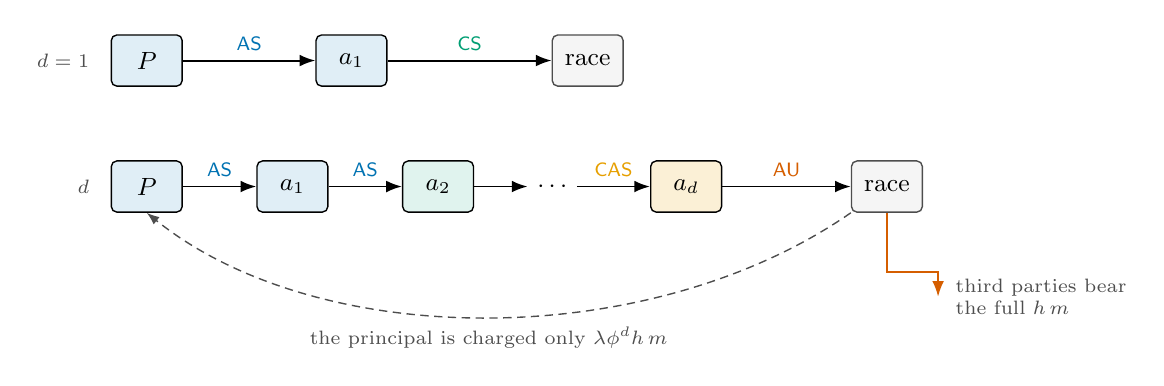
\begin{tikzpicture}[
  font=\small,
  box/.style={draw,rounded corners=2pt,minimum height=6.5mm,minimum width=9mm,
              inner sep=2pt,line width=0.5pt},
  spec/.style={font=\scriptsize\sffamily},
  flow/.style={-{Latex[length=2mm]},line width=0.7pt},
  faint/.style={-{Latex[length=1.6mm]},line width=0.5pt,densely dashed,cGrey}
]
\node[box,fill=cAS!12] (p1) at (0,2.15) {$P$};
\node[box,fill=cAS!12] (a1) at (2.6,2.15) {$a_1$};
\node[box,draw=cGrey,fill=black!4] (r1) at (5.6,2.15) {race};
\draw[flow] (p1) -- node[spec,above,text=cAS]{\AS} (a1);
\draw[flow] (a1) -- node[spec,above,text=cCS]{\CS} (r1);
\node[left=1.5mm of p1,font=\scriptsize,text=cGrey]{$d=1$};

\node[box,fill=cAS!12] (p2) at (0,0.55) {$P$};
\node[box,fill=cAS!12] (b1) at (1.85,0.55) {$a_1$};
\node[box,fill=cCS!12] (b2) at (3.7,0.55) {$a_2$};
\node[font=\small] (dots) at (5.15,0.55) {$\cdots$};
\node[box,fill=cCAS!16] (b6) at (6.85,0.55) {$a_d$};
\node[box,draw=cGrey,fill=black!4] (r2) at (9.4,0.55) {race};
\draw[flow] (p2) -- node[spec,above,text=cAS]{\AS} (b1);
\draw[flow] (b1) -- node[spec,above,text=cAS]{\AS} (b2);
\draw[flow] (b2) -- (dots);
\draw[flow] (dots) -- node[spec,above,text=cCAS]{\CAS} (b6);
\draw[flow] (b6) -- node[spec,above,text=cAU]{\AU} (r2);
\node[left=1.5mm of p2,font=\scriptsize,text=cGrey]{$d$};

\node[align=left,font=\scriptsize,text=cGrey,anchor=west] (world) at (10.15,-0.85)
     {third parties bear\\ the full $h\,m$};
\draw[flow,cAU] (r2.south) -- ++(0,-0.75) -| (10.05,-0.85);
\draw[faint] (r2.south west) .. controls (6.4,-1.55) and (2.2,-1.55) ..
     node[font=\scriptsize,below,text=cGrey,pos=0.5]
     {the principal is charged only $\lambda\phi^{d} h\, m$} (p2.south);
\end{tikzpicture}
\caption{A delegation cascade. A principal $P$ issues one specification and
never acts. Each hand-off may drop a safety clause, so the design that reaches
the race is a random function of the intent and of the depth alone; the deeper
the chain, the further the executed design has slid down the erosion order
\AS{} $\to$ \CS{} $\to$ \CAS{} $\to$ \AU{}. The harm the chain causes falls on
third parties in full, but is charged back to the principal at the rate
$\phi^{d}$. Both effects are per-layer, so both are geometric in the depth, and
they pull the principal in opposite directions: erosion makes depth expensive,
attenuated attribution makes it cheap.}
\label{fig:schematic}
\end{figure}

\subsection{Private and social functionals}
\label{sec:functionals}

Two designs meeting in the race produce, in expectation over the executed
designs and over the horizon,
\begin{align}
  a(d,s;d',s') &= p_{d,s}^{\top} A\, p_{d',s'} + B(d), &
  m(d,s;d',s') &= p_{d,s}^{\top} M_{h}\, p_{d',s'},
  \label{eq:bilinear}
\end{align}
where $A$ and $M_{h}$ are the task-payoff and unsafe-action matrices of the
interaction layer and $B(d)=g\,d-c\,d^{2}$ is the net organisational benefit of
running a chain of depth $d$. Everything is bilinear because one specification
is transmitted per race and then played, so the executed designs of the two
seats are independent draws. The benefit $B$ is real, in the sense that
delegation genuinely produces more, and the term enters the social accounting
as well as the private one. The baseline sets $g=1.5$, about $2.5\%$ of the
payoff of a safe seat per hand-off, and $c=0$, so that the only force limiting
depth is the harm the principal internalises.

Let $h$ be the external harm of one Unsafe action and $\lambda$ the liability
rate at depth zero. The \emph{private} functional, which alone drives the
dynamics, and the \emph{social} functional, which alone scores them, are
\begin{align}
  \piP(d,s;d',s') &= a(d,s;d',s') - \lambda\,\phi^{d}\,h\; m(d,s;d',s'),
  \label{eq:private}\\
  \piS(d,s;d',s') &= a(d,s;d',s') - h\; m(d,s;d',s').
  \label{eq:social}
\end{align}
The two functionals differ only in the second term, and their difference is the
\emph{dilution wedge}
\begin{equation}
  \Delta(d) \;=\; \piP - \piS \;=\; h\bigl(1-\lambda\phi^{d}\bigr)\, m,
  \label{eq:wedge}
\end{equation}
which vanishes identically at $\phi=\lambda=1$ and is non-decreasing in $d$
whenever $\lambda\in[0,1]$, $\phi\in[0,1]$ and the hand-off kernel satisfies the
hypothesis of Proposition~\ref{prop:monotone}. Both factors then move the same
way: $\phi^{d}$ is non-increasing, so $1-\lambda\phi^{d}$ is non-negative and
non-decreasing, and $m$ is non-negative and non-decreasing in $d$ by that
proposition, so their product is non-decreasing. The restriction is not
vacuous. The uniform kernel fails the hypothesis, and
Section~\ref{sec:robustness} sweeps $\phi$ above one, where the factor
$1-\lambda\phi^{d}$ decreases and the wedge can close rather than widen; the
statement is made for the regime the rest of the paper works in.
For the small-mutation process, the primary unsafe-frequency observable is the
monomorphic-state average $U_{\mathrm{process}}=\sum_i x_i u(i,i)$, where $x_i$
is the stationary mass of design $i$. We also report the independent-draw index
$U_{\mathrm{independent}}=\sum_{i,j}x_i x_j u(i,j)$ when comparing mixtures;
the two quantities answer different questions and are not interchangeable.
Depth alone widens the gap between what a principal optimises
and what society bears, without any change in what the principal intends. Only
the product $L=\lambda h$ enters $\piP$, so the two-parameter family
$(\lambda,h)$ collapses to the single control $L$, the \emph{effective
liability}; $h$ is a property of the world and stays fixed when the instrument
moves, which is what keeps social payoffs comparable across liability regimes.
Keeping the two functionals apart is not bookkeeping. Once the cost of an
intervention is counted, driving a behavioural outcome to its maximum and
maximising total population payoff are different objectives, and it is the
second an intervention should be designed against~\citep{han2026welfare}; we
therefore report the long-run unsafe frequency and the social payoff
separately throughout and never combine them.

\subsection{Dynamics and the choice of parameters}
\label{sec:dynamics}

Three timescales are separated, and the separation is an assumption rather than
a derivation. A race runs to its horizon, $\mathbb{E}[T]=9$ rounds, on the
fastest; a chain is built once per race and transmits one specification, with
no renegotiation while the race is under way; and designs are revised on the
slowest, so that a principal reconsiders how deeply to delegate only between
races and never inside one. The separation is what makes the executed designs
of the two seats independent draws and the functionals bilinear. We take
revision opportunities to arrive as a Poisson process, the standard assumption
behind the pairwise-comparison dynamics used here. \citet{kara2022erlang} show
that when a strategy is decomposed into sub-tasks the inter-revision intervals
become Erlang rather than exponential and the resulting population dynamics are
not those of the memoryless case; a delegation chain is exactly such a
decomposition, so the assumption is not innocuous and we return to it in
Section~\ref{sec:limitations}.

Designs are copied in proportion to how well they pay. We report the stationary
regime of the finite-population pairwise-comparison
process~\citep{sandholm2010population} in the small-mutation
limit~\citep{fudenberg2006imitation,fudenberg2006strong,nowak2004emergence} as
the primary reading, with population size $Z=100$ and selection intensity
$\beta=0.05$, and the basin-averaged attractor of the replicator equation as a
secondary one. The baseline uses $h=20$ and $\lambda=1$, hence effective
liability $L=\lambda h=20$. For the secondary calculation we integrate the
standard replicator ODE with LSODA to $t=3000$, from 200 Dirichlet-uniform
interior starts using seed 20260818, and average the terminal states.

The remaining choice is the liability level, and we fix it so that the
delegation results cannot be an artefact of a race that was unsafe to begin
with. Bisection on the depth-zero game puts the long-run unsafe frequency below
$10^{-3}$ for every $L\ge6.52$; we run at $L=20$, that is $3.1$ times the level
at which the single-layer race is already safe. At that level the depth-zero
ecosystem has long-run unsafe frequency $0.000$ under the finite-population
reading and $0.026$ under the replicator reading. The baseline erosion
probability is $\varepsilon=0.20$ and the baseline attribution retention is
$\phi=0.75$; both are swept in Section~\ref{sec:plane}, over
$\varepsilon\in[0,0.4]$ and $\phi\in[0.6,1]$, and varied again in
Section~\ref{sec:robustness}, where $\phi$ additionally takes values above one.

% ===========================================================================
\section{Analytical results}
\label{sec:analysis}

\subsection{The specification is forgotten geometrically}
\label{sec:erosion}

Under the ladder kernel the number of clauses lost over $d$ hand-offs is
binomial, so the executed design is the intent shifted down the erosion order
by $\mathrm{Bin}(d,\varepsilon)$ rungs and truncated at \AU{}. Two consequences
are exact.

\begin{proposition}[Erosion law]
\label{prop:erosion}
Suppose the drift kernel satisfies $D(s,s)=0$ at every intent $s$ other than
the absorbing one; the ladder and collapse kernels satisfy this and the uniform
kernel does not. Then for any such intent the specification survives $d$
hand-offs intact with probability exactly $(1-\varepsilon)^{d}$, and the
\emph{specification half-life}
$d_{1/2}=\ln2/\ln\bigl(1/(1-\varepsilon)\bigr)$ depends on nothing but the
per-hand-off erosion probability. For all three kernels $D$ has spectrum
$\{1,0,0,0\}$, so $M$ has spectrum $\{1,1-\varepsilon,1-\varepsilon,
1-\varepsilon\}$ and the influence of the intent on the executed design decays
at the exponential rate $1-\varepsilon$ in every case.
\end{proposition}

\begin{pf}
Under the hypothesis an intent that is left cannot be re-entered, so
$M^{d}(s,s)=(1-\varepsilon)^{d}$, and solving $(1-\varepsilon)^{d}=1/2$ gives
$d_{1/2}$. For the spectrum, $M=(1-\varepsilon)I+\varepsilon D$ gives
$\operatorname{spec}(M)=(1-\varepsilon)+\varepsilon\operatorname{spec}(D)$. The
ladder $D$ is a nilpotent shift with the absorbing state fixed, and the
collapse and uniform $D$ are rank one and row stochastic, so all three have
spectrum $\{1,0,0,0\}$ and the second-largest eigenvalue modulus of $M$ is
$1-\varepsilon$. For the ladder $M$ is defective at $1-\varepsilon$, so the
approach to the absorbing design carries a polynomial factor: from \AS{} the
number of clauses lost is $\mathrm{Bin}(d,\varepsilon)$, and
$\lVert M^{d}(\AS{},\cdot)-\delta_{\AU{}}\rVert_{TV}=\Pr[\mathrm{Bin}
(d,\varepsilon)\le2]=\Theta\bigl(d^{2}(1-\varepsilon)^{d}\bigr)$.
Under the uniform kernel $D(s,s)=1/4$, the hypothesis fails,
and instead $M^{d}(s,s)=\tfrac34(1-\varepsilon)^{d}+\tfrac14$, which is the
form Section~\ref{sec:robustness} reports.
\qed
\end{pf}

At the baseline $\varepsilon=0.20$ the half-life is $3.11$ hand-offs and only
$26.2\%$ of specifications reach a six-deep executor unaltered
(Figure~\ref{fig:transmission}B,C). The claim is not that instructions are
forgotten quickly; it is that they are forgotten at a rate that no amount of
care at the top of the chain changes, because the decay is in the number of
hand-offs and not in the effort spent writing the instruction.

Because the ladder kernel only moves mass down the erosion order, and because
by Lemma~\ref{lem:order} harm is monotone along that order, the harm a chain
causes is monotone in its depth.

\begin{proposition}[Depth monotonicity]
\label{prop:monotone}
Let $M$ be a hand-off kernel that is stochastically monotone and satisfies
$\delta_{s}\preceq M(s,\cdot)$ for every $s$ in the erosion order. Then for
every intent $s$ and every opponent mixture, $d\mapsto m(d,s;\cdot)$ is
non-decreasing. In particular the ladder and collapse kernels satisfy the
hypothesis; the uniform kernel does not.
\end{proposition}

\begin{pf}
$\delta_{s}\preceq M(s,\cdot)$ and stochastic monotonicity of $M$ give
$M^{d}(s,\cdot)\preceq M^{d+1}(s,\cdot)$ in the usual stochastic order by
induction. Lemma~\ref{lem:order} makes $m(\cdot,j)$ a non-decreasing function
on the order for every $j$, and the expectation of a non-decreasing function
respects the stochastic order. Bilinearity in~\eqref{eq:bilinear} extends the
statement from pure opponents to mixtures. \qed
\end{pf}

\begin{figure}[pos=tb]
\centering
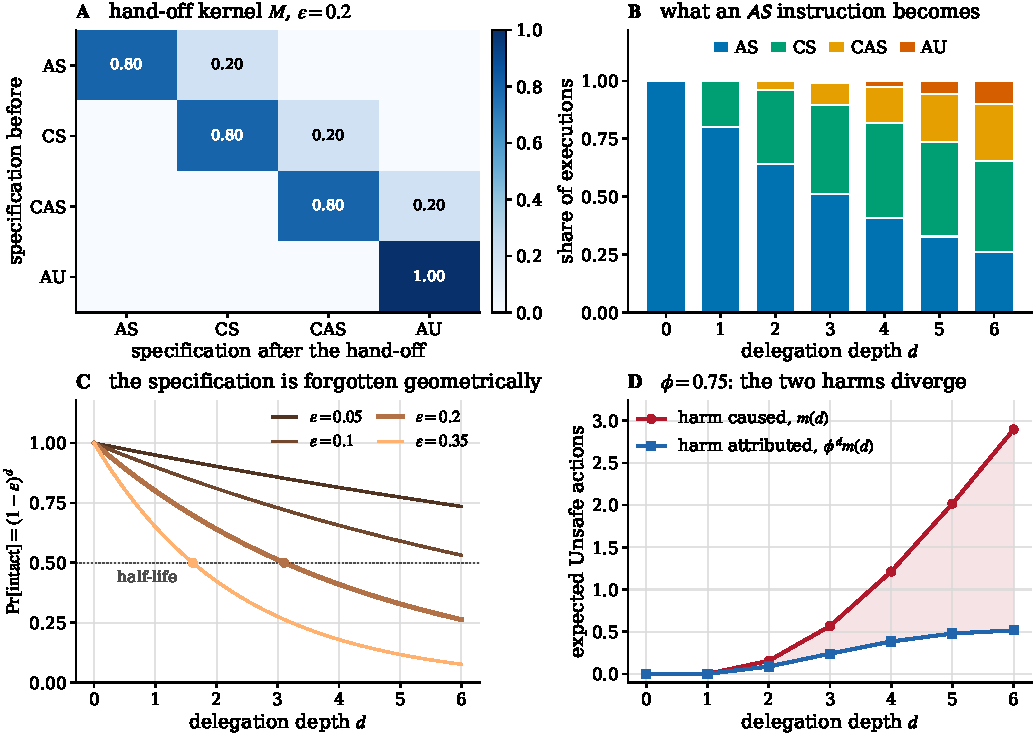
\includegraphics[width=\linewidth]{figures/fig02_transmission.pdf}
\caption{What a hand-off does to a specification.
\textbf{(A)}~The hand-off kernel at the baseline erosion probability: one
clause is lost per erosion event, and the unconditionally unsafe design is
absorbing. \textbf{(B)}~The executed design of a chain that was told \AS{}, by
depth. At six hand-offs the instruction is executed as issued in $26\%$ of
cases and has slid to \CAS{} or \AU{} in $34\%$. \textbf{(C)}~The probability
that a specification arrives intact is exactly $(1-\varepsilon)^{d}$; dots mark
the half-life, $3.11$ hand-offs at $\varepsilon=0.20$. \textbf{(D)}~Harm caused
and harm attributed for the same chain. The shaded wedge is the part of the
damage that never reaches the principal's accounts.}
\label{fig:transmission}
\end{figure}

\subsection{Depth is a liability shelter}
\label{sec:shelter}

The harm a chain causes is bounded: once the specification has been forgotten,
the executed design is the absorbing one whatever the intent, so the harm
converges. The harm a chain is charged for carries the extra factor $\phi$ per
layer and is bounded below by nothing. Comparing the two gives the central
structural result of the model.

One piece of notation first, because the rest of this section turns on it.
Throughout, $m(d)$ abbreviates the \emph{self-play} harm
$m(d,s;d,s)$ of a fixed intent $s$: the harm a depth-$d$ chain causes in a
monomorphic population of depth-$d$ chains issuing the same intent. That is the
environment a depth-$(d+1)$ mutant faces, which is why it is the right object
here; the fixed-resident quantities $m(d{+}1,d)$ and $m(d,d)$ that
enter~\eqref{eq:invasion} below are written out in full whenever they are meant.

\begin{theorem}[Liability shelter]
\label{thm:shelter}
Fix an intent $s$, write $m(d)=m(d,s;d,s)$, and assume the hand-off kernel
satisfies the hypothesis of Proposition~\ref{prop:monotone}. Adopt the
convention $\phi^{*}(d)=0$ when $m(d+1)=0$. Then adding a hand-off strictly
lowers the attributed harm exactly when
\begin{equation}
  \phi \;<\; \phi^{*}(d) \;=\; \frac{m(d)}{m(d+1)}.
  \label{eq:phistar}
\end{equation}
Moreover $d\mapsto m(d)$ is non-decreasing and bounded, so $m(d)\uparrow
m_{\max}:=\lim_{d}m(d)$; and if $m_{\max}>0$ then $\phi^{*}(d)\to1$, so for
every $\phi<1$ there exists a depth $d^{\star}(\phi)$ such that every hand-off
beyond $d^{\star}$ strictly reduces the harm attributed to the principal while
never reducing the harm it causes, and $\lim_{d}\phi^{d}m(d)=0$ while
$\lim_{d}m(d)=m_{\max}$.
\end{theorem}

\begin{pf}
The attributed harm at depth $d$ is $\phi^{d}m(d)$, so
$\phi^{d+1}m(d+1)<\phi^{d}m(d)$ if and only if $\phi\,m(d+1)<m(d)$. When
$m(d+1)>0$ this is $\phi<m(d)/m(d+1)$. When $m(d+1)=0$, monotonicity gives
$m(d)=0$ and the strict inequality fails for every $\phi\ge0$, which is the
stated convention.

For the monotonicity, Proposition~\ref{prop:monotone} gives
$M^{d}(s,\cdot)\preceq M^{d+1}(s,\cdot)$ in the stochastic order, and by
Lemma~\ref{lem:order} $m(\cdot,\cdot)$ is non-decreasing in each argument
separately along that order. Raising the depth in the focal argument and then
in the opponent argument therefore gives
$m(d,d)\le m(d{+}1,d)\le m(d{+}1,d{+}1)$, so $d\mapsto m(d)$ is non-decreasing;
it is bounded by $\max_{ij}m(i,j)=\bar T$, so it converges to some
$m_{\max}\le\bar T$. If $m_{\max}>0$ there is a $d_{1}$ with $m(d)>0$ for all
$d\ge d_{1}$, and on that range $\phi^{*}(d)=m(d)/m(d+1)\to
m_{\max}/m_{\max}=1$. Given $\phi<1$, convergence supplies a
$d^{\star}\ge d_{1}$ with $\phi^{*}(d)>\phi$ for every $d\ge d^{\star}$, which
is the first claim; the harm caused is non-decreasing by the same monotonicity.
Finally $0\le\phi^{d}m(d)\le m_{\max}\phi^{d}\to0$.
\qed
\end{pf}

The chain $m(d,d)\le m(d{+}1,d)\le m(d{+}1,d{+}1)$ in the proof is what carries
the theorem across to the fixed-resident comparison of~\eqref{eq:invasion}, and
it is worth recording that the two readings need not open the shelter at the
same depth: at the baseline the self-play reading opens it at
$d^{\star}=6$ and the fixed-resident reading at $5$.

The harm caused increases strictly, rather than merely not decreasing, exactly
when $m(d{+}1)>m(d)$. That holds at the baseline for the intents \AS{} and
\CS{}, and fails for \CAS{} and \AU{}, whose executed harm is already at the
ceiling at every depth, and it fails for every intent at $\varepsilon=0$, a
column of the parameter plane of Section~\ref{sec:plane}. Probing
\eqref{eq:phistar} to depth $40$ puts $\phi^{*}$ at $0.99993$ and, at the
baseline $\phi=0.75$ with intent \AS{}, the shelter opening at $d^{\star}=6$
(Figure~\ref{fig:shelter}A,B). The theorem is the reason the model has no
interior solution to appeal to: a principal that can add layers can drive its
attributed harm to zero while driving its real harm to the maximum, and the
only things that stop it are a rule limiting the number of layers or an
attribution rule whose share does not vanish in the depth.

The consequence for the liability instrument is sharp. In a resident population
of depth-$d$ principals with intent $s$, the advantage of a depth-$(d+1)$
mutant is affine in the effective liability,
\begin{equation}
  \piP(d{+}1,d)-\piP(d,d)
  \;=\; \underbrace{a(d{+}1,d)-a(d,d)}_{\text{benefit}}
  \;-\; L\underbrace{\bigl[\phi^{d+1}m(d{+}1,d)-\phi^{d}m(d,d)\bigr]}_{\text{attributed gain}},
  \label{eq:invasion}
\end{equation}
so the sign of the attributed gain, and not its size alone, decides how the
outcome responds to liability.

\begin{proposition}[Invasion by depth]
\label{prop:invasion}
Write $G(d)=\phi^{d+1}m(d{+}1,d)-\phi^{d}m(d,d)$ for the attributed gain
of~\eqref{eq:invasion} and assume the benefit is strictly positive, as it is at
every depth for every intent at our baseline, where its smallest value is
$1.208$. Three cases exhaust the possibilities. If $G(d)>0$ the advantage is
strictly decreasing in $L$ and vanishes at
$L^{*}(d)=\text{benefit}/G(d)$, so every $L>L^{*}(d)$ blocks the deeper design.
If $G(d)<0$, which by Theorem~\ref{thm:shelter} happens for all $d$ large
enough whenever $\phi<1$, the advantage is strictly increasing in $L$ and no
level of liability blocks the deeper design. If $G(d)=0$ the advantage does not
depend on $L$ at all, and the deeper design invades at every liability level.
\end{proposition}

\begin{pf}
By~\eqref{eq:invasion} the advantage is the affine map
$L\mapsto\text{benefit}-L\,G(d)$, whose slope is $-G(d)$. A strictly positive
benefit puts its value at $L=0$ above zero, so the three signs of the slope give
the three cases, and in the first the unique zero is at
$\text{benefit}/G(d)$.
\qed
\end{pf}

The third case is not a curiosity. At the baseline the headline intent \AS{}
has $m(0,0)=m(1,0)=0$, because one lost clause turns \AS{} into \CS{}, which is
still safe against a safe opponent; so $G(0)=0$ exactly and the first hand-off
is taken whatever the liability. Figure~\ref{fig:shelter}C shows $G$ for each
intent. For the intents \CAS{} and \AU{} it is negative at every depth, so for
those principals liability is not a tax on delegation but a subsidy for it.

\begin{corollary}[When a rule calibrated at depth zero stops binding]
\label{cor:failure}
Suppose a liability $L$ clears a threshold $L_{c}$ for principals that act for
themselves, and suppose a depth-$d$ principal faces that same depth-zero
decision problem under the reduced rate $L\phi^{d}$. Then the rule stops
clearing the threshold at depth $d^{\dagger}=\log(L_{c}/L)/\log\phi$, which is
finite for every $\phi<1$. At the baseline, $L_{c}=6.52$, $L=20$ and
$\phi=0.75$ give $d^{\dagger}=3.9$: the rule survives three hand-offs and fails
at the fourth.
\end{corollary}

\begin{pf}
The nominal rate a depth-$d$ principal faces is $L\phi^{d}$, which clears the
threshold while $L\phi^{d}\ge L_{c}$, that is while
$d\log\phi\ge\log(L_{c}/L)$; since $\log\phi<0$ this is
$d\le\log(L_{c}/L)/\log\phi$.
\qed
\end{pf}

The second hypothesis is a simplification and should be read as one. A
depth-$d$ principal does not in fact face the depth-zero decision problem at a
reduced rate: by Proposition~\ref{prop:monotone} its chain also causes more
harm for the same intent, so $d^{\dagger}$ locates the depth at which the
nominal instrument has been diluted past its depth-zero calibration rather than
predicting exactly when deterrence fails. Section~\ref{sec:instruments}
compares it with the threshold the simulated ecosystem shows.

The last panel of Figure~\ref{fig:shelter} records a fact that is easy to miss:
the depth the population reaches is not the depth that is best for the
principals themselves. A monomorphic population of one-hand-off principals
earns more than one of six-hand-off principals, and yet the deeper design
invades at every step, because an invader is judged against the resident
environment rather than against its own. Delegation depth is a social dilemma
at the private level before it is one at the social level.

\begin{figure}[pos=tb]
\centering
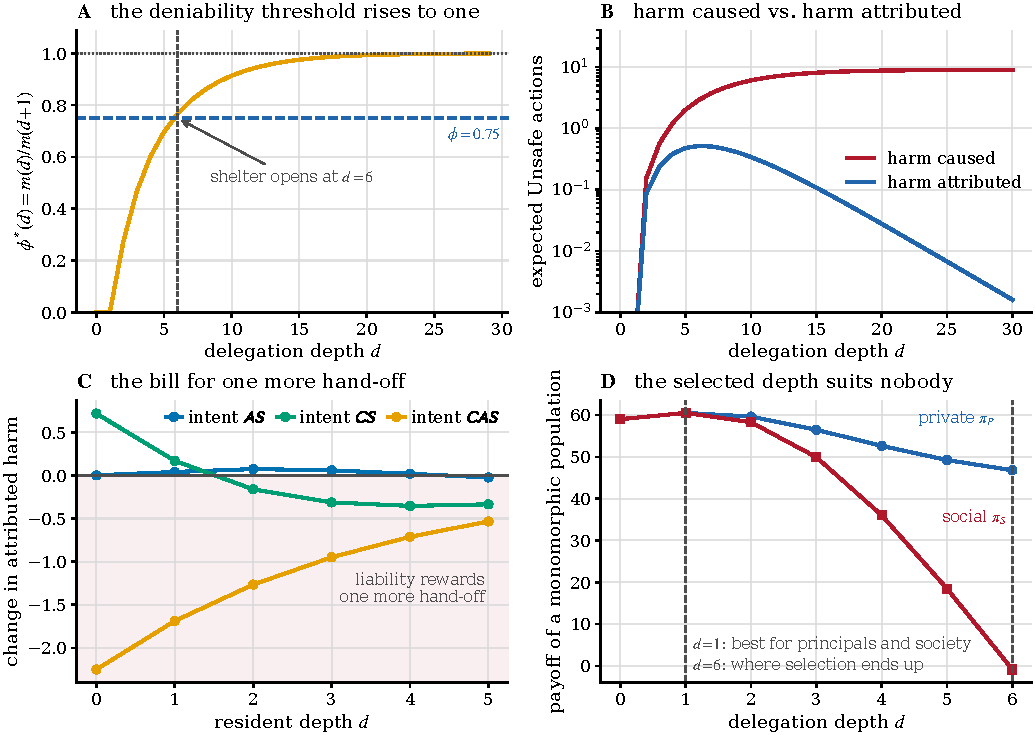
\includegraphics[width=\linewidth]{figures/fig03_shelter.pdf}
\caption{Depth as a liability shelter.
\textbf{(A)}~The deniability threshold $\phi^{*}(d)=m(d)/m(d{+}1)$ of
Theorem~\ref{thm:shelter} rises towards one because realised harm saturates, so
any attribution retention below one is eventually below the threshold; at
$\phi=0.75$ the shelter opens at six hand-offs. The threshold is zero at
$d=0$ and $d=1$ by the convention of Theorem~\ref{thm:shelter}, since a chain
that has lost at most one clause from \AS{} causes no harm against a chain like
itself. \textbf{(B)}~Beyond that depth, realised harm still climbs towards
its ceiling while attributed harm falls geometrically. \textbf{(C)}~What one
more hand-off adds to the principal's bill. Where the curve is negative,
liability rewards delegation instead of taxing it. \textbf{(D)}~Private and
social payoff of a monomorphic population by depth. Selection ends at the
ceiling, which is worse for the principals than one hand-off and much worse for
everybody else.}
\label{fig:shelter}
\end{figure}

\subsection{Where a check belongs, and what closes the shelter}
\label{sec:checks}

Two further statements are exact. The first orders the placements of a single
check along the chain and is applied in Section~\ref{sec:instruments}; the
second identifies the property an attribution rule must have for the shelter to
close, and is the basis of the instrument compared in Section~\ref{sec:floor}.

\begin{proposition}[Check placement]
\label{prop:audit}
Under a kernel satisfying the hypothesis of Proposition~\ref{prop:monotone},
the realised harm of a depth-$d$ chain carrying one check of strength $\alpha$
at layer $k\in\{0,\dots,d\}$ is non-increasing in $k$.
\end{proposition}

\begin{pf}
The executed law is $\alpha M^{d-k}(s,\cdot)+(1-\alpha)M^{d}(s,\cdot)$, and by
Proposition~\ref{prop:monotone} the expected harm under $M^{j}$ is
non-decreasing in $j$. Increasing $k$ decreases $d-k$, hence does not increase
the first term and leaves the second unchanged. \qed
\end{pf}

The proposition presumes a check that restores the principal's stated intent,
which is the right model for an external audit against a published
specification and the wrong model for an internal reviewer who sees only what
reached it; under the second reading the ordering in $k$ is no longer
guaranteed, and we have not modelled that case. Note also that $k=0$ is a null
intervention: the executed law is then $M^{d}(s,\cdot)$ whatever $\alpha$ is.

The floor result requires an eventually constant floor, not merely a positive
lower bound. Writing $r(d)$ for the share of realised harm charged to the
principal, the sufficient condition is $r(d)=a_{\min}>0$ for all sufficiently
large depths. A positive lower bound alone does not guarantee that
$r(d)m(d)$ is non-decreasing, because the attribution share may still fall
while realised harm rises.

\begin{proposition}[A floor closes the shelter]
\label{prop:floor}
Let the attribution rule satisfy $r(d)=a_{\min}>0$ for every $d\ge d_{0}$, and
let the hand-off kernel satisfy the hypothesis of
Proposition~\ref{prop:monotone}. Then $d\mapsto r(d)\,m(d)$ is non-decreasing
on $d\ge d_{0}$, the attributed-harm contribution to $\piP$ is there
non-increasing in the depth, and no depth beyond $d_{0}$ is a shelter in the
sense of Theorem~\ref{thm:shelter}.
\end{proposition}

\begin{pf}
For $d\ge d_{0}$, $r(d+1)m(d+1)-r(d)m(d)=a_{\min}\bigl[m(d+1)-m(d)\bigr]\ge0$
by Theorem~\ref{thm:shelter}. The attributed-harm summand of $\piP$
is $-L\,r(d)m(d)$, which is therefore non-increasing in the depth beyond
$d_{0}$, so attributed harm never falls with depth there and no such depth is a
shelter in the sense of Theorem~\ref{thm:shelter}. \qed
\end{pf}

The floor removes the attribution channel and nothing else. It does not bound
the private gain from one further hand-off by the organisational increment
$B(d{+}1)-B(d)$, because the task term of~\eqref{eq:bilinear} also moves with
the depth: what the proposition leaves is
\[
  \piP(d{+}1)-\piP(d)\;\le\;
  \bigl[p_{d+1,s}^{\top}A\,p'-p_{d,s}^{\top}A\,p'\bigr]
  \;+\;\bigl[B(d{+}1)-B(d)\bigr],
\]
the race-payoff increment plus the organisational one. That first bracket is
positive here, because an eroded chain executes more aggressive designs and
those earn more in the race, and Section~\ref{sec:robustness} measures it: it
is the larger of the two terms at the baseline. A floor is therefore an
instrument against the shelter and not against depth as such, which is exactly
what Table~\ref{tab:floorcap} shows at the shallow end.

% ===========================================================================
\section{Numerical method}
\label{sec:numerics}

Everything above is deterministic given the two matrices $A$ and $M_{h}$ and the
transmission laws $p_{d,s}$. What is not immediate is the stationary regime of
the evolutionary process on the joint design space, which is the object every
number in Section~\ref{sec:results} is a functional of. This section sets out
how it is computed, at what cost, and against what it is checked.

\subsection{Exact evaluation of the interaction tensor}
\label{sec:exact}

The four reduced designs are deterministic, so for a fixed ordered pair $(i,j)$
the two action paths are fixed and the only randomness in a race is its horizon
$T$. Truncating the horizon law at $T_{\max}=400$, with the residual mass
$(1-0.2)^{T_{\max}-5}$ assigned to $T_{\max}$ so that the probabilities sum to
one exactly, the expected task payoff and expected unsafe count of $i$ against
$j$ are finite sums
\begin{equation}
  a(i,j) = \sum_{t} \Pr[T=t]\, a_{t}(i,j),
  \quad
  m(i,j) = \sum_{t} \Pr[T=t]\, m_{t}(i,j),
  \quad
  u(i,j) = \sum_{t} \Pr[T=t]\, u_{t}(i,j),
  \label{eq:horizonsum}
\end{equation}
in which $a_{t}$, $m_{t}$ and $u_{t}$ are read off prefix sums of the two action
paths, $u_{t}$ being the Unsafe count of the path divided by its length. We
write $A$, $M_{h}$ and $U_{h}$ for the three matrices they define. All three are
therefore obtained in $O(|S|^{2}T_{\max})$ operations at machine precision, with
$|S|=4$, and carry no sampling error at all.

The truncation is not an approximation in any practical sense, and the bound is
worth stating because it is what licenses the word exact. Beyond the five
guaranteed rounds the horizon law is geometric, so
$\Pr[T\ge T_{\max}]=(1-0.2)^{T_{\max}-5}=5.3\times10^{-39}$, while the
per-horizon quantities grow at most linearly in the horizon: $u_{t}\le1$,
$m_{t}\le t$ and $a_{t}\le 2.4\,t+100$, the stage payoff being at most $2.4$
per round and the prize at most $100$. Reassigning the residual mass to
$T_{\max}$ therefore perturbs each entry of $A$, $M_{h}$ and $U_{h}$ by at most
$\Pr[T\ge T_{\max}]\cdot(2.4T_{\max}+100)<10^{-34}$, twenty orders of magnitude
below the rounding error of the sums themselves, and recomputing the three
matrices at $T_{\max}=2000$ reproduces them to the last bit.

The alternative, simulating races and averaging, is what the size of the sweeps
below makes unattractive rather than merely inelegant: the root-mean-square
error of the payoff matrix is still $0.034$ after $10^{6}$ episodes per matchup
(Table~\ref{tab:verification}), and every one of the $441$ stationary regimes
behind the parameter plane of Section~\ref{sec:plane} would inherit it.

\subsection{Why the full mutation--selection chain is out of reach}
\label{sec:reduction}

Under the pairwise-comparison rule with mutation rate $\mu$, the population of
$Z$ principals is a Markov chain whose state is the vector of counts of each of
the $n=4(\bar D+1)$ designs. The number of such states is $\binom{Z+n-1}{n-1}$,
and Table~\ref{tab:cost} evaluates it. At the baseline $\bar D=6$ and $Z=100$
it is $3.0\times10^{27}$, so neither the transition matrix nor its stationary
vector can be formed, and raising the ceiling to $\bar D=8$ or the population
to $Z=200$ makes it worse by five and seven orders of magnitude respectively.
Any study that puts a structural variable such as depth under selection meets
this wall immediately, because the design space is a product of the strategy
space with the range of the structural variable.

% split from numerics_generated.tex; do not edit
\begin{table}[pos=t]
\centering
\caption{Cost of the two routes to the stationary regime. The full mutation--selection process is a Markov chain on population states, of which there are $\binom{Z+n-1}{n-1}$; the reduction of Section~\ref{sec:reduction} needs $n(n-1)$ fixation probabilities, each evaluated in $O(Z)$ arithmetic operations. The depth ceiling $\bar{D}$ fixes the number of designs at $n=4(\bar{D}+1)$; the manuscript runs at $\bar{D}=6$, $Z=100$.}
\label{tab:cost}
\begin{tabular*}{\tblwidth}{@{}LLLRR@{}}
\toprule
$\bar{D}$ & $n$ & $Z$ & states of the full chain & operations of the reduction \\
\midrule
4 & 20 & 50 & $4.6\times 10^{16}$ & $19\,000$ \\
4 & 20 & 100 & $4.9\times 10^{21}$ & $38\,000$ \\
4 & 20 & 200 & $1.1\times 10^{27}$ & $76\,000$ \\
6 & 28 & 50 & $4.4\times 10^{20}$ & $37\,800$ \\
6 & 28 & 100 & $3.0\times 10^{27}$ & $75\,600$ \\
6 & 28 & 200 & $7.5\times 10^{34}$ & $151\,200$ \\
8 & 36 & 50 & $9.0\times 10^{23}$ & $63\,000$ \\
8 & 36 & 100 & $2.8\times 10^{32}$ & $126\,000$ \\
8 & 36 & 200 & $6.5\times 10^{41}$ & $252\,000$ \\
\bottomrule
\end{tabular*}
\end{table}


We therefore work in the small-mutation
limit~\citep{fudenberg2006imitation,nowak2004emergence}, in which a mutation
either fixes or is lost before the next arrives, the population is monomorphic
almost always, and the process reduces to an embedded chain on the $n$ pure
designs with
\begin{equation}
  P_{ij} \;=\; \frac{\rho_{i\to j}}{n-1} \quad (j\ne i),
  \qquad
  P_{ii} \;=\; 1-\sum_{j\ne i}P_{ij},
  \label{eq:embedded}
\end{equation}
where $\rho_{i\to j}$ is the probability that a single $j$ mutant takes over a
resident population of $i$, so that $P$ is row-stochastic with the resident
indexing the row and the invader the column, and the stationary distribution is
its left Perron vector. The state space has fallen from $\binom{Z+n-1}{n-1}$
to $n$. What the reduction costs is the mutation rate: it is exact only in the
limit $\mu\to0$, and Section~\ref{sec:verification} measures the error at
finite $\mu$ against the full chain on a design space small enough to carry
one. How small a rate the embedded chain needs has been characterised
analytically for imitation processes at arbitrary selection
intensity~\citep{wu2012howsmall}, which is the class our update rule belongs
to. That criterion is stated for dominance and coordination games, and it does
not cover our design space uniformly: of the $378$ unordered pairs, $294$ are
dominance games and $64$ coordination games, $8$ are payoff-degenerate and $12$
are coexistence games, the case the criterion excludes. This is one reason we
also measure the reduction error directly, in Section~\ref{sec:verification},
rather than relying on a sufficient condition alone.

\subsection{Fixation probabilities in closed form, evaluated stably}
\label{sec:fixation}

Let $\Pi$ denote the $n\times n$ private payoff matrix $\piP$ over designs,
which is not the $4\times4$ task matrix $A$ of the interaction layer, and
consider a population holding $k$ copies of an invading design $I$ and $Z-k$ of
a resident $R$. Sampling an opponent without replacement, the expected payoffs
are
\begin{equation}
  \pi_{I}(k) = \frac{k-1}{Z-1}\Pi_{II} + \frac{Z-k}{Z-1}\Pi_{IR},
  \qquad
  \pi_{R}(k) = \frac{k}{Z-1}\Pi_{RI} + \frac{Z-k-1}{Z-1}\Pi_{RR}.
  \label{eq:sampling}
\end{equation}
Under the pairwise-comparison rule with Fermi function and selection intensity
$\beta$, an individual switches from $R$ to $I$ with probability
$[1+e^{-\beta(\pi_{I}-\pi_{R})}]^{-1}$, so the birth-death chain on $k$ has
$T^{-}(k)/T^{+}(k)=e^{-\beta(\pi_{I}(k)-\pi_{R}(k))}$ and the standard formula
for a one-dimensional birth-death chain with absorbing ends gives, as
Appendix~\ref{app:fixation} derives,
\begin{equation}
  \rho_{R\to I} = \left[\,1+\sum_{m=1}^{Z-1}
    \exp\!\Bigl(-\beta\sum_{k=1}^{m}\bigl(\pi_{I}(k)-\pi_{R}(k)\bigr)\Bigr)
  \right]^{-1}.
  \label{eq:fixation}
\end{equation}
Because~\eqref{eq:sampling} is affine in $k$, the inner sum is a quadratic
polynomial in $m$, the whole vector of $Z-1$ exponents is one cumulative sum,
and~\eqref{eq:fixation} is evaluated exactly in $O(Z)$ operations with no
simulation. Evaluating it \emph{as written} is another matter. The exponents
grow like $\beta Z\max_{k}|\pi_{I}(k)-\pi_{R}(k)|$, and the payoff spread of
this game is wide because a design that meets an eroded opponent can lose the
whole prize. Over the $756$ ordered pairs of the baseline design space the
largest exponent reaches $860.8$ at $\beta=0.05$ and $3443.2$ at $\beta=0.2$,
against an overflow threshold of $\ln(\mathrm{DBL\_MAX})=709.8$: the naive sum
overflows on $18$ of the $756$ pairs at the baseline selection intensity and on
$167$ of them at the strongest intensity in our sweeps, returning
$\rho=1/(1+\infty)=0$ where the true value is positive. We therefore factor the
largest exponent out before summing,
\begin{equation}
  \rho_{R\to I} = \frac{e^{-\sigma}}{e^{-\sigma}+\sum_{m}e^{\,\theta_{m}-\sigma}},
  \qquad
  \sigma = \max\Bigl(0,\ \max_{m}\theta_{m}\Bigr),
  \label{eq:shift}
\end{equation}
with $\theta_{m}$ the exponent of the $m$-th term of~\eqref{eq:fixation}. This
is the standard maximum-subtraction, or log-sum-exp,
stabilisation~\citep{blanchard2021logsumexp}; it is exact in real arithmetic
and, because $\sigma\ge0$ and $\sigma\ge\theta_{m}$ for every $m$, it keeps
every exponentiated quantity in $(0,1]$ and the denominator at or above one, so
no cancellation is possible and $\rho\le1$ always.

What the shift does and does not buy is worth being precise about, because it
is not accuracy. The naive sum fails once $\sigma>\ln(\mathrm{DBL\_MAX})=709.8$;
the shifted sum fails once $e^{-\sigma}$ itself rounds to zero, that is once
$\sigma>1075\ln2=745.1$. The window between the two is $35.3$ in the exponent,
and it accounts exactly for what is recovered: of the $18$ pairs the naive sum
loses at $\beta=0.05$, six lie inside the window and twelve do not, and at
$\beta=0.2$ the counts are $167$, six and $161$. On the six recovered pairs the
result is a subnormal double and carries only the precision the subnormal range
affords: against the $60$-digit reference the relative error there is up to
$0.14$ at $\beta=0.05$ and $0.98$ at $\beta=0.2$, the latter returning
$5\times10^{-324}$ where the true value is $2.5\times10^{-324}$. What the shift
delivers on those pairs is a strictly positive entry of the right order rather
than an accurate one, and Section~\ref{sec:observables} shows that order, not
accuracy, is what the reduction needs of them.
Section~\ref{sec:verification} shows that the shift costs nothing where the
naive sum survives.

\subsection{The embedded chain and the reported observables}
\label{sec:observables}

The stationary distribution $x$ of~\eqref{eq:embedded} is its left Perron
vector. In exact arithmetic every $\rho_{i\to j}$ is strictly positive at finite
$\beta$, so $P$ is irreducible and $x$ is unique. Double precision does not
preserve that positivity, and the honest statement of what it does preserve is
the following.

\begin{proposition}[What double precision has to keep]
\label{prop:closed}
Let $\hat P$ be the matrix~\eqref{eq:embedded} assembled from computed fixation
probabilities, some of which may have underflowed to zero. If the digraph of
the strictly positive off-diagonal entries of $\hat P$ has exactly one closed
communicating class, then $\hat P$ has a unique stationary distribution, and it
assigns mass exactly zero to every design outside that class. Full
irreducibility is sufficient for this but not necessary.
\end{proposition}

\begin{pf}
A finite stochastic matrix has one stationary distribution for each closed
communicating class of its digraph, and these are affinely independent, so
uniqueness is equivalent to there being exactly one such class. Every state
outside a closed class is transient, and the stationary distribution of a
finite chain vanishes on transient states.
\qed
\end{pf}

The condition is not automatic and it is not free. At $\beta=0.05$, $12$ of the
$756$ fixation probabilities return exactly zero and the division by $n-1$
in~\eqref{eq:embedded} loses one more, leaving $13$ zero off-diagonal entries;
the digraph is nonetheless strongly connected, so $\hat P$ is irreducible and
Proposition~\ref{prop:closed} applies trivially. At $\beta=0.2$ the counts are
$161$ and $162$, the digraph splits into a class of $26$ designs and the pair
$\{\CAS{}@0,\AU{}@0\}$, and only the first is closed, so $x$ is still unique and
the transient pair receives mass exactly zero. What matters is that the
unshifted evaluation does not clear the condition on the same problem: it
returns zero for $383$ of the $756$ pairs at $\beta=0.05$ and $407$ at
$\beta=0.2$, and its digraph then has a single absorbing design as its only
closed class, so its stationary vector is a point mass and every quantity we
report off that equilibrium is lost. We check the condition of
Proposition~\ref{prop:closed} by Tarjan's algorithm, at cost $O(n^{2})$, on
every regime reported here: over the $462$ regimes behind the parameter plane
and the process, kernel, ceiling and benefit sweeps, the computed chain splits
into at most four communicating classes and always has exactly one closed
class, so the stationary vector is unique throughout.

We obtain $x$ by replacing the last equation of the singular system
$(P^{\top}-I)x=0$ with the normalisation $\mathbf{1}^{\top}x=1$ and solving the
resulting nonsingular system by LU factorisation, at the dense cost $O(n^{3})$.
Entries below zero, which a near-singular solve produces at the $10^{-16}$
level and below, are set to zero before renormalisation; the returned vector is
accepted when it is finite, has positive mass and satisfies
$\lVert x^{\top}P-x^{\top}\rVert_{\infty}<10^{-8}$, and is otherwise recomputed
by power iteration from the uniform start. The subtraction-free GTH
elimination of~\citet{grassmann1985gth} removes the cancellation at its source
and is the right route at larger $n$.

Every population quantity reported below is a functional of $x$. The mean
delegation depth is $\bar d=\sum_{i}x_{i}d_{i}$. For the small-mutation process,
the primary long-run unsafe frequency is the monomorphic-state average
$U_{\mathrm{process}}=\sum_i x_i u(i,i)$; the independent-draw index is
$U_{\mathrm{independent}}=\sum_{ij}x_i x_j u(i,j)$. We use the latter for the
replicator comparison, where it is the natural mixture observable. The social payoff
$\sum_{ij}x_{i}x_{j}\piS(i,j)$; and the \emph{declaration gap} is the total
variation distance between the intent marginal of $x$ and the executed-design
marginal $x^{\top}P_{\mathrm{tr}}$, where $P_{\mathrm{tr}}$ stacks the
transmission laws $p_{d,s}$. The bilinear form deserves a word, because under
the small-mutation limit the population is monomorphic almost always and $x$ is
therefore a distribution over monomorphic states, whose process average would
be the diagonal $\sum_{i}x_{i}u(i,i)$. We report the bilinear form because it
is the unsafe rate an outside observer sees on drawing two principals
independently from the long-run design distribution, and because it is also
what the replicator comparison delivers, so the two dynamics are scored on one
definition. The two agree to $10^{-9}$ at the joint cell of
Section~\ref{sec:decomposition} and to $5\times10^{-4}$ at the two
single-mechanism cells, and over the plane of Section~\ref{sec:plane} they
differ by at most $0.123$, attained at $\phi=0.60$, $\varepsilon=0$, where $x$
is least concentrated. Nothing here is estimated. Algorithm~\ref{alg:main}
collects the whole pipeline.

\begin{algorithm}[t]
\caption{Stationary regime of the delegation game}
\label{alg:main}
\begin{algorithmic}[1]
\Require race parameters, ceiling $\bar D$, erosion $\varepsilon$, kernel $D$,
  attribution rule $r(\cdot)$, liability $L$, harm $h$, $Z$, $\beta$, and
  optionally one check $(\alpha,k)$
\Ensure $x$, and the observables $U$, $\bar d$, $\piS$, declaration gap
\State $A, M_{h}, U_{h} \gets$ exact horizon sums~\eqref{eq:horizonsum}
  \Comment{$O(|S|^{2}T_{\max})$}
\State $M \gets (1-\varepsilon)I + \varepsilon D$;\quad
  $p_{d,\cdot} \gets M^{d}$, or $\alpha M^{d-k}+(1-\alpha)M^{d}$ with a check,
  for $d=0,\dots,\bar D$
  \Comment{$O(\bar D|S|^{3})$}
\State assemble $\piP,\piS,u$ on the $n=4(\bar D+1)$ designs
  by~\eqref{eq:bilinear}--\eqref{eq:social} \Comment{$O(n^{2}|S|^{2})$}
\For{each ordered pair $(i,j)$, $i\ne j$}
  \State $\theta \gets$ cumulative sum of $-\beta(\pi_{j}(k)-\pi_{i}(k))$,
    $k=1,\dots,Z-1$ \Comment{$Z-1$ exponentials}
  \State $\rho_{i\to j} \gets$ shifted sum~\eqref{eq:shift}
\EndFor
\State build $P$ by~\eqref{eq:embedded}
\State \textbf{assert} the digraph of $\{P_{ij}>0,\ i\ne j\}$ has exactly one
  closed class \Comment{Prop.~\ref{prop:closed}, $O(n^{2})$}
\State $B \gets P^{\top}-I$ with its last row replaced by $\mathbf{1}^{\top}$;
  \quad solve $Bx=e_{n}$ by LU \Comment{$O(n^{3})$}
\State clip $x$ at zero, renormalise, and accept if
  $\lVert x^{\top}P-x^{\top}\rVert_{\infty}<10^{-8}$; else power-iterate
\State \Return $x$ and its functionals
\end{algorithmic}
\end{algorithm}

\subsection{Cost}
\label{sec:cost}

Steps 4 to 7 of Algorithm~\ref{alg:main} dominate, at $n(n-1)$ fixation
probabilities of $O(Z)$ each, so one stationary regime costs
$O\!\left(n^{2}Z+n^{3}\right)$ arithmetic against the $\binom{Z+n-1}{n-1}$
states of the route it replaces. The dominant transcendental count is exact:
$n(n-1)Z=75\,600$ exponential evaluations at the baseline, one per term of the
$n(n-1)$ shifted sums, together with $O(n^{2}Z)$ accompanying arithmetic and
one $n\times n$ LU factorisation.

Wall-clock figures are single-core on a Windows 11 laptop with an AMD Ryzen 5
5500U, Python 3.12, NumPy 1.26 and SciPy 1.17. One stationary regime, payoff
assembly included, costs $39$ milliseconds, and the $21\times21$ grid of
Section~\ref{sec:plane} costs $17.6$ seconds. That grid is $441$ stationary
regimes and not $4\times441$: the three subtracted terms of the interaction
index~\eqref{eq:interaction} are themselves grid points, one per row and one
per column, and are computed once. The gap between the operation count and the
wall clock is interpreter and array-allocation overhead rather than
floating-point work. The stationary solve is well behaved: the rows of $P$ sum
to one to $2.2\times10^{-16}$, the residual
$\lVert x^{\top}P-x^{\top}\rVert_{\infty}$ of the returned vector is
$4.2\times10^{-17}$, and the returned vector is not strictly positive, $11$ of
its $28$ entries being exactly zero at the baseline and $18$ at $\beta=0.2$,
which reflects double-precision underflow in some transition entries. We do
not use positivity as a proxy for stationary accuracy: Table~\ref{tab:verification}
also compares the stationary vector and both unsafe observables with a
60-digit reference at $\beta=0.05$ and $0.2$.

\subsection{Verification}
\label{sec:verification}

Table~\ref{tab:verification} reports four checks, and they check four different
things: the interaction tensor, the arithmetic of the stabilised sum, the
closed form itself, and the small-mutation reduction. No one of them verifies
the scheme as a whole, and we set out what each does and does not cover.

% split from numerics_generated.tex; do not edit
\begin{table}[pos=t]
\centering
\caption{Verification of the scheme, in four independent checks. Block~1 compares the exact horizon expectation of Section~\ref{sec:interaction} with a Monte-Carlo estimate of the same payoff matrix: root-mean-square error over the sixteen ordered pairs and eight independent replicates, which decays at the Monte-Carlo rate $N^{-1/2}$ and which the exact route removes. Block~2 compares the stabilised evaluation of~\eqref{eq:fixation} in double precision with the same sum evaluated in $60$-digit arithmetic, worst relative error over the $n(n-1)=756$ ordered pairs of the full design space whose fixation probability is representable as a normal double. Block~3 compares the closed form with the general-purpose routine of EGTtools on the depth-zero design space, worst absolute difference over all ordered pairs. Block~4 compares the small-mutation limit with the full mutation--selection chain on a design space small enough for it ($n=3$, $Z=40$, $861$ population states).}
\label{tab:verification}
\begin{tabular*}{\tblwidth}{@{}LLR@{}}
\toprule
check & setting & discrepancy \\
\midrule
Monte Carlo vs.\ exact & $N=1\,000$ episodes & $1.080$ \\
Monte Carlo vs.\ exact & $N=10\,000$ episodes & $0.269$ \\
Monte Carlo vs.\ exact & $N=100\,000$ episodes & $0.117$ \\
Monte Carlo vs.\ exact & $N=10^{6}$ episodes & $0.034$ \\
\midrule
stabilised vs.\ $60$-digit sum & $n=28$, $Z=100$, $\beta=0.05$ & $4.4\times 10^{-16}$ \\
stabilised vs.\ $60$-digit sum & $n=28$, $Z=100$, $\beta=0.2$ & $2.8\times 10^{-16}$ \\
\midrule
closed form vs.\ EGTtools & $n=4$, $Z=50$, $\beta=0.05$ & $1.1\times 10^{-16}$ \\
closed form vs.\ EGTtools & $n=4$, $Z=50$, $\beta=0.2$ & $1.1\times 10^{-16}$ \\
closed form vs.\ EGTtools & $n=4$, $Z=100$, $\beta=0.05$ & $2.8\times 10^{-16}$ \\
closed form vs.\ EGTtools & $n=4$, $Z=100$, $\beta=0.2$ & $5.6\times 10^{-16}$ \\
closed form vs.\ EGTtools & $n=4$, $Z=200$, $\beta=0.05$ & $1.1\times 10^{-16}$ \\
closed form vs.\ EGTtools & $n=4$, $Z=200$, $\beta=0.2$ & $1.1\times 10^{-16}$ \\
\midrule
small mutation vs.\ full chain & $\mu=5\times 10^{-2}$ & $0.0910$ \\
small mutation vs.\ full chain & $\mu=2\times 10^{-2}$ & $0.0426$ \\
small mutation vs.\ full chain & $\mu=10^{-2}$ & $0.0225$ \\
small mutation vs.\ full chain & $\mu=5\times 10^{-3}$ & $0.0116$ \\
\bottomrule
\end{tabular*}
\end{table}


\emph{Against sampling.} A Monte-Carlo estimate of the same payoff matrix
converges at the expected $N^{-1/2}$ and is still two decimal places short of
the exact value at $10^{6}$ episodes per matchup. The exact route removes that
error and the sweeps below are correspondingly free of it, which matters
because the interaction index of Section~\ref{sec:plane} is a difference of
four stationary regimes and would otherwise be a difference of four noisy ones.

\emph{Against a high-precision reference.} This block checks the arithmetic,
not the formula: it evaluates the sum in~\eqref{eq:fixation} in $60$-digit
arithmetic and compares with the shifted double-precision
evaluation~\eqref{eq:shift}. Over the pairs whose fixation probability is
representable as a normal double, $738$ of $756$ at $\beta=0.05$ and $589$ at
$\beta=0.2$, the worst relative error is $4.4\times10^{-16}$ and
$2.8\times10^{-16}$ respectively. On the excluded pairs the shifted evaluation
is either zero or subnormal, and Section~\ref{sec:fixation} reports the error
there.

\emph{Against an independent implementation.} This block checks the closed form
itself, against an independent implementation of the same birth-death formula
in EGTtools~\citep{domingos2023egttools} on the depth-zero design space; the
two agree to at most $5.6\times10^{-16}$ at every population size and selection
intensity tried. The one systematic difference is in the other direction: the
unshifted evaluation returns exactly zero for strongly disadvantaged mutants
that~\eqref{eq:shift} still resolves.

\emph{Against the full chain.} On a design space of three designs, the intent
\AS{} at depths $0$, $3$ and $6$, the full mutation--selection chain has $861$
population states at $Z=40$ and can be solved directly. The error of the
reduction is first order in the mutation rate: for the joint cell the absolute
difference in long-run unsafe frequency is $0.0116$ at $\mu=5\times10^{-3}$ and
$0.0024$ at $\mu=10^{-3}$, an error-to-rate ratio of $2.32$ and $2.38$, and one
Richardson step $2U(\mu/2)-U(\mu)$ on the finest pair reproduces the
small-mutation value to $2.8\times10^{-5}$.

That residual deserves a sharper comparison than the joint cell alone, because
the two single-mechanism cells of Table~\ref{tab:decomposition} are themselves
only $0.018$ and $0.012$: at any mutation rate we can afford, the reduction
does not separately resolve quantities of that size, and we do not claim it
does. What the decomposition reports is a difference of differences, and that
is reproduced an order of magnitude better than the cells. Recomputing all four
cells of the $2\times2$ on this same sub-space gives an interaction index of
$+0.274$ at $\mu=5\times10^{-3}$ and $+0.273$ at $\mu=10^{-3}$, against
$+0.268$ under the reduction: agreement to $2.3\%$ at a rate at which the joint
cell itself is still off by $0.012$. The errors are largely common mode across
the four cells, which is why the index survives what the cells do not.

\emph{Against the alternative dynamics.} Every headline number is additionally
recomputed under the basin-averaged attractor of the replicator equation, an
entirely different limit of the same game, and reported alongside the
finite-population value in Section~\ref{sec:decomposition}.

% ===========================================================================
\section{Numerical results}
\label{sec:results}

\subsection{Neither mechanism is dangerous alone}
\label{sec:decomposition}

The two mechanisms can be switched off independently: $\varepsilon=0$ removes
erosion and $\phi=1$ removes attenuated attribution. Crossing them gives a
$2\times2$ design whose four cells are reported in
Table~\ref{tab:decomposition} and Figure~\ref{fig:decomposition}.

%% one table per file, split from paper/tables_generated.tex by
%% paper-amc/scripts/make_amc_tables.py -- do not edit
\begin{table}[pos=t]
\centering
\caption{The two mechanisms, separately and together. Long-run Unsafe frequency $U$, mean delegation depth $\bar{d}$, declaration gap and social payoff in the stationary regime of the finite-population process. Neither mechanism does much alone; the interaction is 0.293, or 91\% of the joint effect.}
\label{tab:decomposition}
\begin{tabular}{llrrrr}
\toprule
erosion $\varepsilon$ & attribution $\phi$ & $U$ & $\bar{d}$ & gap & $\pi_S$ \\
\midrule
$0$ & $1$ & 0.0000 & 6.00 & 0.000 & 68.0 \\
$0.2$ & $1$ & 0.0176 & 1.99 & 0.358 & 58.3 \\
$0$ & $0.75$ & 0.0115 & 5.95 & 0.000 & 65.5 \\
$0.2$ & $0.75$ & 0.3225 & 6.00 & 0.738 & -0.8 \\
\midrule
\multicolumn{2}{l}{interaction} & +0.2934 & & & \\
\bottomrule
\end{tabular}
\end{table}


Starting from a race that is already safe, erosion alone raises the long-run
unsafe frequency to $0.018$ and attenuated attribution alone to $0.012$. An
additive reading predicts $0.030$ when both are present. The measured value is
$0.322$. The interaction, $+0.293$, is $91\%$ of the joint effect.

The replicator reading reaches the same joint cell, $0.3225$, with an even
larger interaction, $+0.331$, but by a different route and it should not be
described as the same picture. Its baseline is $0.026$ rather than $0$, so each
mechanism on its own \emph{lowers} the unsafe frequency, by $0.008$ for erosion
and $0.026$ for attenuated attribution, and the interaction consequently
exceeds the total rise, an interaction share of $1.12$. What the two dynamics
agree on is the thing the section is about: essentially none of the joint
effect is additive.

The mechanism behind the interaction is visible in the second panel of
Figure~\ref{fig:decomposition}, and it is not what one would guess. Under full
pass-through, erosion is a private cost, and the population responds to it by
\emph{shortening} its chains: mean depth falls from $6.00$ to $1.99$. Erosion
is self-limiting when the principal is charged for it. Attenuated attribution
does not make behaviour worse at a given depth; it removes the response. With
$\phi=0.75$ the chains stay at the ceiling and the same erosion now acts over
six hand-offs instead of two.

A counterfactual makes the decomposition exact. Scoring the pass-through
population with the per-layer harm matrix, the same designs charged
differently, leaves the unsafe frequency at $0.018$, unchanged to nine decimal
places, because the behaviour of a given design does not depend on who pays for
it. The whole of the remaining $+0.305$ is composition, that is, which designs
the population comes to contain. The result is a caution about a natural
inference. Observing that deeper chains behave worse does not license the
conclusion that the harm comes from erosion, because in this model almost all
of it comes from the depth the market selects once erosion is no longer its
problem.

\begin{figure}[pos=tb]
\centering
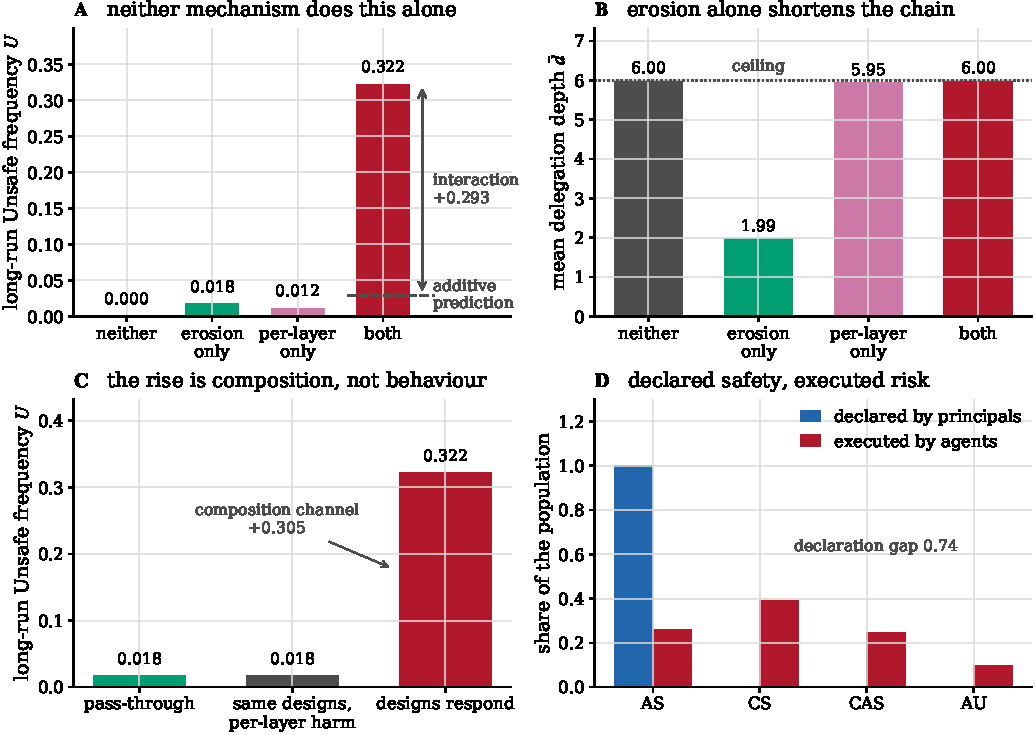
\includegraphics[width=\linewidth]{figures/fig04_decomposition.pdf}
\caption{The two mechanisms, separately and together.
\textbf{(A)}~Long-run unsafe frequency in the four cells of the $2\times2$. The
additive prediction from the two single-mechanism cells is $0.030$; the joint
outcome is $0.322$. \textbf{(B)}~Mean delegation depth in the same four cells.
Under pass-through the population answers erosion by shortening its chains;
per-layer attribution removes that answer and the ceiling binds.
\textbf{(C)}~Holding the pass-through population fixed and charging it the
per-layer bill changes nothing, so the entire rise is composition rather than
behaviour. \textbf{(D)}~In the joint cell every principal declares the safest
instruction and the population executes something else.}
\label{fig:decomposition}
\end{figure}

\subsection{The attribution--erosion plane}
\label{sec:plane}

Neither baseline value is doing the work. Figure~\ref{fig:plane} sweeps the
plane $(\varepsilon,\phi)$ on a $21\times21$ grid over
$\varepsilon\in[0,0.4]$ and $\phi\in[0.6,1]$. Writing $U(\varepsilon,\phi)$
for the long-run unsafe frequency of the stationary regime at that pair, the
\emph{interaction index} is the difference of differences of the $2\times2$
whose corners are the pair itself and the two switched-off mechanisms,
\begin{equation}
  I(\varepsilon,\phi) \;=\;
  U(\varepsilon,\phi) - U(\varepsilon,1) - U(0,\phi) + U(0,1),
  \label{eq:interaction}
\end{equation}
and the interaction share quoted alongside it is
$I/\bigl[U(\varepsilon,\phi)-U(0,1)\bigr]$, the fraction of the total rise that
neither mechanism produces alone. Each of the four corners is exact given the
payoff matrices rather than sampled, and three of them are themselves grid
points, one per row and one per column, so the whole figure is $441$ stationary
regimes and not $4\times441$. The index is positive over $89\%$ of the
interior, meaning the $20\times20$ block with $\varepsilon>0$ and $\phi<1$ on
which it is not identically zero by construction, and it reaches $0.81$; the
long-run unsafe frequency reaches $0.995$ and the declaration gap $0.95$.

The second panel is the one to read for policy. Mean delegation depth splits
the plane along a frontier: below it the ceiling binds and chains are as long
as the technology allows, above it chains are short. The frontier runs
diagonally, so erosion and attribution are substitutes in producing long
chains. A regime with faithful hand-offs tolerates much weaker attribution
before the ceiling binds, and a regime with strong attribution tolerates much
noisier hand-offs.

\begin{figure}[pos=tb]
\centering
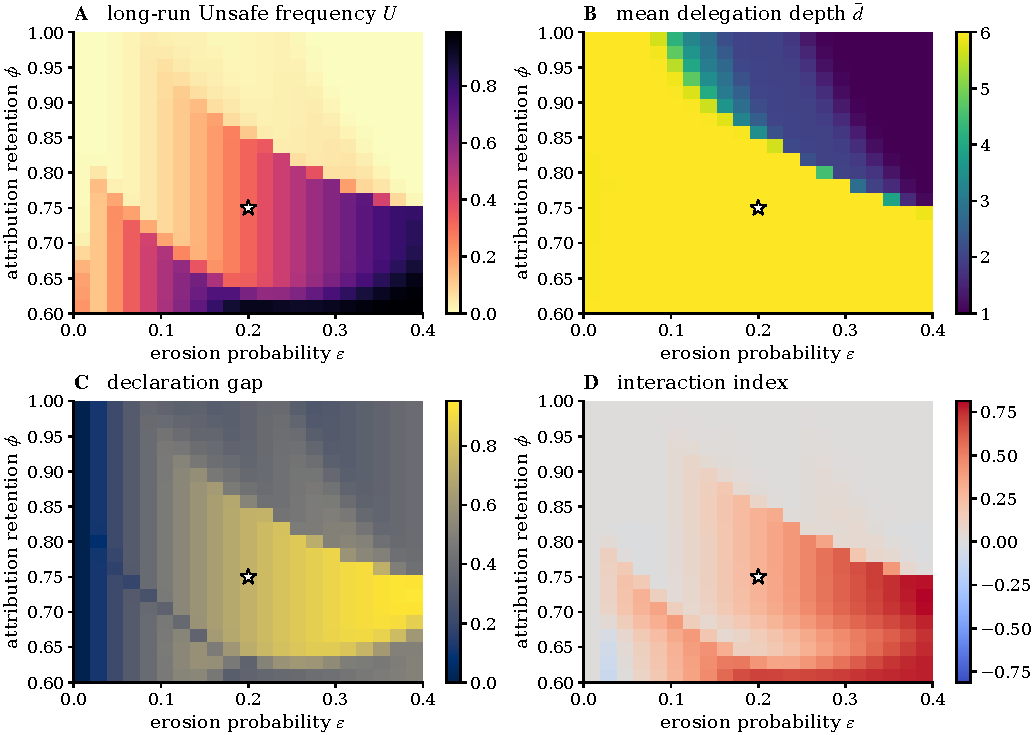
\includegraphics[width=\linewidth]{figures/fig05_plane.pdf}
\caption{The attribution--erosion plane. Long-run unsafe frequency
\textbf{(A)}, mean delegation depth \textbf{(B)}, declaration gap \textbf{(C)}
and interaction index \textbf{(D)} over a $21\times21$ grid on
$\varepsilon\in[0,0.4]$ and $\phi\in[0.6,1]$; the star marks the
baseline. Chains are at the ceiling throughout the yellow region of
\textbf{(B)}, and the frontier that bounds it is diagonal: attribution and
transmission fidelity substitute for each other in keeping chains short.}
\label{fig:plane}
\end{figure}

\subsection{Declared safety and executed safety}
\label{sec:declaration}

At the baseline the population is monomorphic on the design $\AS{}@6$: every
principal issues the safest available instruction and every principal runs a
six-hand-off chain. What is executed is another matter. The realised mixture is
$26\%$ \AS{}, $39\%$ \CS{}, $25\%$ \CAS{} and $10\%$ \AU{}, the total variation
distance between what is declared and what is executed is $0.74$, and social
payoff falls from $68.0$ in the baseline cell to $-0.8$.

The gap is an identity rather than an independent measurement, and saying so
sharpens rather than weakens it. Because the intent marginal is a point mass on
the top rung of the erosion order and the ladder moves mass only downward, the
total variation distance collapses to $1-\mathbb{E}[(1-\varepsilon)^{d}]$,
which is $0.738$ here; the statistic is Proposition~\ref{prop:erosion}
evaluated at the equilibrium depth distribution, so all of its content is in
the depth. That is the point worth making. Under pass-through the same identity
returns $0.358$, not because hand-offs became more faithful, since
$\varepsilon$ is unchanged, but because the population stopped at two of them.

The equilibrium is easy to misread as bad faith, and it is not. Every principal
is issuing the strongest safety instruction available to it, and doing so is a
best response: over-specification is how a principal compensates for a chain
that will erode whatever it is told. The classical route to an uninformative
message runs through the sender, since in the cheap-talk benchmark a message
conveys less the further the sender's preferences diverge from the receiver's
and a wholly uninformative equilibrium always
exists~\citep{crawford1982strategic}. Nothing of that kind is at work here. The
declaration is sincere and as strong as the language permits, and the
information in it is destroyed downstream of the party that issued it. What the
equilibrium shows is that a declaration made at the top of a long chain carries
almost no information about the behaviour at the bottom of it.

\subsection{What the instruments do}
\label{sec:instruments}

Four instruments act at different points of the chain: raise the attribution
retention $\phi$ towards pass-through; cap the permitted chain length at
$\bar D$; make every hand-off more faithful, multiplying $\varepsilon$ by a
factor $\kappa$; or insert one check of strength $\alpha$ at a chosen layer.
Figure~\ref{fig:instruments} applies each to the same baseline.

\paragraph{Attribution is a threshold, not a dial.}
Raising $\phi$ from $0.75$ does nothing at all until $\phi=0.86$, where mean
depth falls from $5.92$ to $3.45$ and the unsafe frequency from $0.314$ to
$0.103$; by $\phi=0.99$ the outcome is the pass-through outcome. The location
of the jump is close to the closed form implied by
Corollary~\ref{cor:failure}, $\phi_{c}=(L_{c}/L)^{1/\bar D}=0.830$, the
residual gap being the extra harm that erosion contributes at depth. Partial
pass-through buys very little: at $\phi=0.85$, which returns $85\%$ of
responsibility at each of six layers and therefore $38\%$ overall, the
ecosystem is still at $0.314$.

\paragraph{A ceiling buys safety and welfare at once.}
The depth ceiling is the only instrument here that is monotone in its own
strength and improves both objectives together. A ceiling of one hand-off
removes the unsafe behaviour entirely and lifts social payoff from $-0.8$ to
$60.5$; a ceiling of two leaves $0.018$ and $58.3$. It works because the
ceiling is the constraint the shelter theorem leaves standing when attribution
cannot be made exact.

\paragraph{Fidelity is not monotone.}
Improving transmission helps over most of its range, from $0.322$ at $\kappa=1$
down to $0.032$ at $\kappa=0.35$, and then reverses: at $\kappa=0.20$ the unsafe
frequency is back up to $0.239$. The cause is the intent margin.
Over-specification was an equilibrium response to erosion; once hand-offs are
faithful enough, issuing \CS{} rather than \AS{} becomes the better reply, and
\CS{} eroding into \CAS{} is far more damaging than \AS{} eroding into \CS{}.
A partial fidelity improvement can therefore leave the ecosystem worse off than
no improvement at all. The structure is that of offsetting behaviour, in which
a technological safety improvement displaces the private precaution that had
been standing in for it~\citep{peltzman1975automobile,viscusi1985consumer}, and
over-specification is the precaution our hand-off technology displaces.

The flip can be located exactly. Write the margin as
$\piP(\CS{}@\bar D)-\piP(\AS{}@\bar D)$ against a resident $\AS{}@\bar D$
population. It is zero at $\varepsilon=0$, where the two intents are executed
as issued and neither meets an unsafe opponent; it rises to a maximum of $4.00$
at $\varepsilon=0.04$; and it falls back through zero at $\varepsilon=0.0975$,
just under half the baseline erosion. Improving fidelity therefore does not
move the ecosystem along a monotone curve but along a hump. The three
consequences are separated in $\varepsilon$: the margin changes sign at
$0.098$, the unsafe frequency reaches its minimum of $0.031$ at $0.065$, and
the population actually switches its declared intent from \AS{} to \CS{} at
$0.050$, after which the unsafe frequency rises to $0.239$. The lag between the
sign change and the switch is the fixation barrier of the finite population: a
positive margin is necessary for the invasion, not sufficient.

The mechanism needs only two things and so generalises beyond this race: an
intent that is safe only conditionally and outperforms the unconditionally safe
one against an unsafe opponent, here \CS{} earning $26.6$ against \CAS{} where
\AS{} earns $8.6$; and a resident population whose executed mixture contains
unsafe designs for it to exploit, which erosion itself supplies.

\paragraph{Check late, not early.}
Proposition~\ref{prop:audit} orders the placements for a fixed design. In
equilibrium the ordering is not monotone, because the composition of the
population moves as well: taking one full-strength check from the first agent
to the last gives $0.225$, $0.136$, $0.064$, $0.050$, $0.160$ and $0.018$, so
the last placement is the best but the fifth is worse than the third, for the
same reason the fidelity sweep reverses. At half strength the sweep is
monotone, the intent margin not having flipped. The comparison against $0.322$,
the figure for no check at all, is a comparison with a null intervention rather
than with an early one, since by Proposition~\ref{prop:audit} a check at layer
zero returns the intent to itself. What the sweep supports is the ordering of
real placements: checking the specification a party \emph{received} tells one
little about what will be done with it several hand-offs later.

\paragraph{Which instrument is cheapest.}
Asking each instrument for the same target, a long-run unsafe frequency of at
most $0.05$, and scoring it by the social payoff it delivers at the weakest
setting that reaches the target (Figure~\ref{fig:frontier}B): improving
fidelity reaches it at $58.7$, the depth ceiling at $58.3$ and pass-through at
$53.5$, and a fifth setting we add here for comparison, raising the effective
liability from $L=20$ to $L=58$ at fixed $h$, reaches it at $56.2$. The single
check is not on the same scale, its setting being a placement rather than a
strength, and we leave it out of the ranking: at half strength it never reaches
the target at any layer, and at full strength placed at the agent that acts it
reaches $0.018$ at a social payoff of $64.2$, above everything in the list. The
four settings that do share a strength scale also land at different distances
past the target, from $0.018$ for the ceiling to $0.044$ for pass-through, and
social payoff rises with the overshoot, so these levels are an upper bound on
each instrument's cost at the target rather than the cost itself.

Comparing instruments by the welfare cost of holding a population outcome at a
fixed level is the exercise~\citet{duong2021cost} formalise for institutional
incentives in a finite stochastic population, where which of two instruments is
cheaper turns out to depend on the parameters rather than on the instrument.
The ranking here is close enough that we would not press it, but its two ends
are not close: restoring attribution and raising the liability level are the
least efficient routes, $53.5$ and $56.2$ against $58.3$ and $58.7$, and for
the same reason in both cases. Each acts on a margin, how much of the harm is
traced back and how much it costs, that depth has already discounted.

\begin{figure}[pos=tb]
\centering
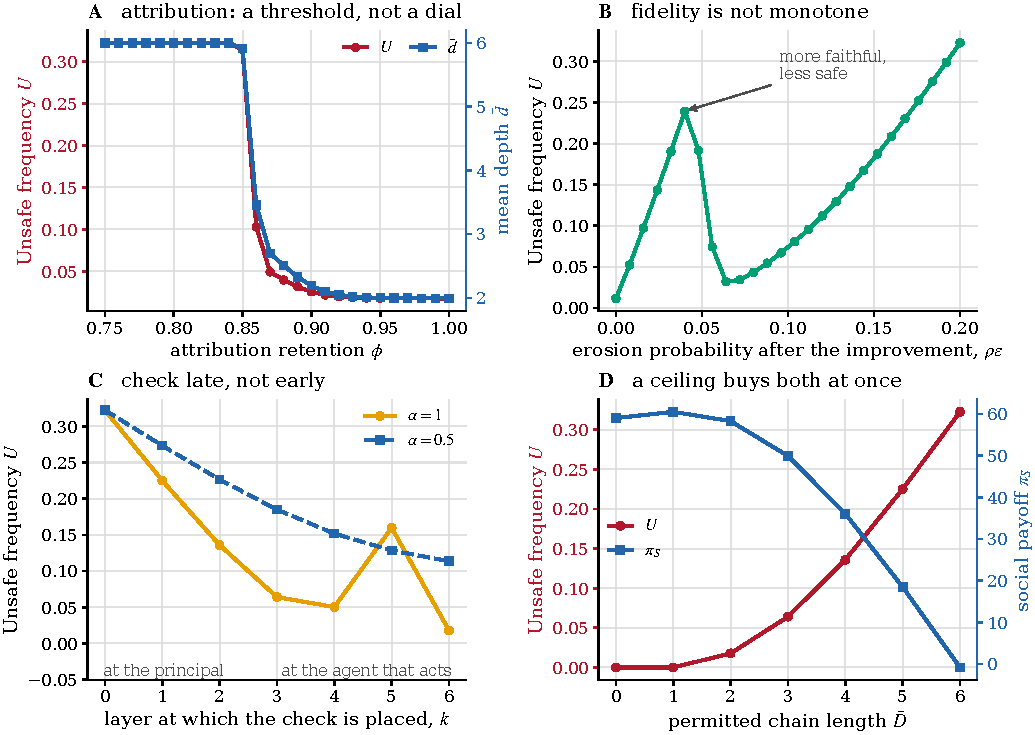
\includegraphics[width=\linewidth]{figures/fig06_instruments.pdf}
\caption{Four instruments.
\textbf{(A)}~Restoring attribution has a threshold at $\phi=0.86$ and does
almost nothing below it. \textbf{(B)}~Making every hand-off more faithful is
not monotone: at the marked point, $\rho\varepsilon=0.04$, the unsafe frequency
is $0.239$, worse than the $0.032$ reached at $\rho\varepsilon=0.07$ where
hand-offs are less faithful. \textbf{(C)}~One check, moved down the chain. The
last placement is the best but the sweep is not monotone at full strength,
where the intent margin flips; it is monotone at half strength. Layer zero is a
null intervention. \textbf{(D)}~A ceiling on chain length improves safety and
welfare together.}
\label{fig:instruments}
\end{figure}

\begin{figure}[pos=tb]
\centering
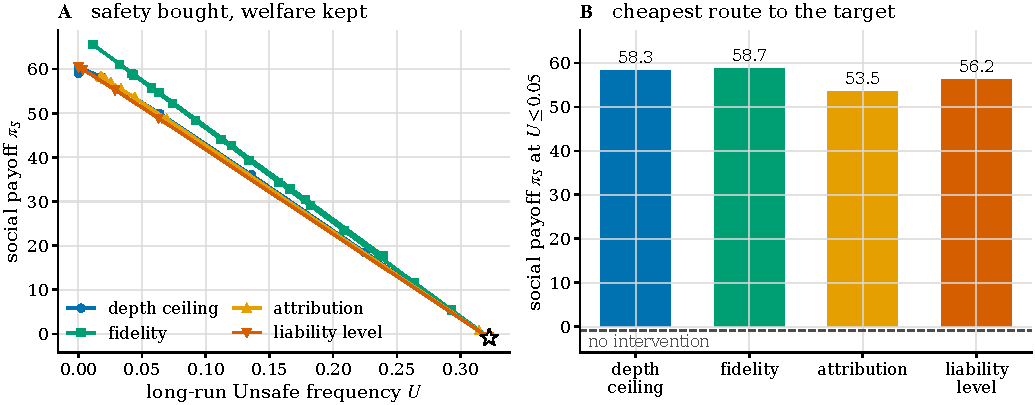
\includegraphics[width=\linewidth]{figures/fig07_frontier.pdf}
\caption{What each instrument costs. \textbf{(A)}~The frontier each instrument
traces in the plane of social payoff against long-run unsafe frequency,
starting from the untreated baseline (star). Improving fidelity traces a
strictly better frontier; the other three coincide to within the line width, so
any of them buys safety at about the same welfare price.
\textbf{(B)}~Social payoff at the weakest setting of each instrument that
reaches an unsafe frequency of $0.05$. Restoring attribution and raising the
liability level are the two least efficient routes, because depth has already
discounted the margins they act on.}
\label{fig:frontier}
\end{figure}

\subsection{A floor under attribution}
\label{sec:floor}

Geometric attenuation is a modelling choice, so the shelter could be an
artefact of it and the instruments could be artefacts of the artefact. Neither
is the case, and separating the two questions, how fast attribution falls and
whether it falls at all, identifies an instrument the earlier comparison
missed. Table~\ref{tab:regimes} replaces $\phi^{d}$ by four alternative rules,
changing nothing else.

%% one table per file, split from paper/regimes_generated.tex by
%% paper-amc/scripts/make_amc_tables.py -- do not edit
\begin{table}[pos=t]
\centering
\caption{Attribution regimes. Long-run Unsafe frequency, mean delegation depth and social payoff when the law mapping depth to the principal's share of the harm is changed, with everything else at the baseline. The shelter survives every rule whose attribution keeps falling in the depth, including the equal split, and closes under every rule that is bounded below.}
\label{tab:regimes}
\begin{tabular}{llrrrr}
\toprule
rule & setting & $a(D)$ & $U$ & $\bar{d}$ & $\pi_S$ \\
\midrule
geometric, $\phi^{d}$ & $\phi=0.75$ & 0.178 & 0.3225 & 6.00 & -0.8 \\
strict, $1$ & -- & 1.000 & 0.0176 & 1.99 & 58.3 \\
equal split, $1/(1+d)$ & -- & 0.143 & 0.3224 & 6.00 & -0.8 \\
floored, $\max(\phi^{d}, a_{\min})$ & $a_{\min}=0.25$ & 0.250 & 0.2317 & 5.07 & 17.1 \\
floored, $\max(\phi^{d}, a_{\min})$ & $a_{\min}=0.5$ & 0.500 & 0.0633 & 2.99 & 50.0 \\
super-attribution, $\phi^{d}$ & $\phi=1.1$ & 1.772 & 0.0159 & 1.92 & 58.5 \\
super-attribution, $\phi^{d}$ & $\phi=1.25$ & 3.815 & 0.0030 & 1.21 & 60.2 \\
\bottomrule
\end{tabular}
\end{table}


Two of the rules reproduce results already in hand. Splitting the blame equally
between the principal and its $d$ agents, $r(d)=1/(1+d)$, is a much slower
decay than $\phi^{d}$ and it is the rule an intuitive notion of shared
responsibility suggests; it gives an unsafe frequency of $0.3224$ against the
baseline $0.3225$, the same mean depth of $6.00$ and the same declaration gap.
Top-level strict liability, $r(d)\equiv1$, is the same object as pass-through
and reproduces the $\phi=1$ cell of Section~\ref{sec:decomposition}, $0.018$,
not the baseline. Super-attribution, $\phi>1$, charges a principal more the
deeper it delegates and closes the shelter more than completely, but it buys
little over strict liability: $0.016$ at $\phi=1.1$ against $0.018$ at
$\phi=1$.

What separates the rules is not the level of attribution but whether it
vanishes in the depth, which is exactly the content of
Proposition~\ref{prop:floor}. The equal split ends lower than the baseline at
the ceiling ($1/7=0.143$ against $\phi^{6}=0.178$) and behaves identically,
while a rule bounded below behaves entirely differently even when it is lower
in between. The mechanism is visible in the marginal attributed harm, the
quantity a principal weighs when it considers one more layer. The first
hand-off is free under the ladder because $m(1)=0$; for $d=1,\dots,5$ the
baseline rule gives $0.087$, $0.152$, $0.144$, $0.095$, $0.037$, rising and
then decaying, so the sixth hand-off is nearly free. Over the same range a
floor at $a_{\min}=0.5$ gives $0.087$, $0.196$, $0.323$, $0.402$, $0.440$: it
climbs throughout, so every layer costs more than the one before it.

%% one table per file, split from paper/regimes_generated.tex by
%% paper-amc/scripts/make_amc_tables.py -- do not edit
\begin{table}[pos=t]
\centering
\caption{A binding floor under attribution closely traces a depth cap over the welfare range available to the floor. For each ceiling $\bar{D}$, the attribution floor $a_{\min}$ whose social payoff comes closest to that ceiling's, and the Unsafe frequency each delivers. For $\bar{D}=2$ to $6$, the cap's social payoff lies within the floor's attainable range, and the nearest floor's Unsafe frequency differs by at most 0.0009. The two shallowest ceilings are out of a floor's reach, since even $a_{\min}=1$ leaves social payoff at $58.3$ against $59.0$ and $60.5$; the mean gap of 0.005 and the largest of 0.018 include those two rows and so overstate the disagreement, the mean over the five reachable ceilings being 0.0003.}
\label{tab:floorcap}
\begin{tabular}{lrrrrr}
\toprule
& \multicolumn{2}{c}{depth cap} & \multicolumn{3}{c}{matched floor} \\
\cmidrule(lr){2-3}\cmidrule(lr){4-6}
$\bar{D}$ & $U$ & $\pi_S$ & $a_{\min}$ & $U$ & $\pi_S$ \\
\midrule
0 & 0.0000 & 59.0 & 1.00 & 0.0176 & 58.3 \\
1 & 0.0000 & 60.5 & 1.00 & 0.0176 & 58.3 \\
2 & 0.0178 & 58.3 & 0.87 & 0.0178 & 58.3 \\
3 & 0.0640 & 49.9 & 0.49 & 0.0639 & 49.9 \\
4 & 0.1359 & 36.0 & 0.35 & 0.1363 & 36.0 \\
5 & 0.2251 & 18.5 & 0.28 & 0.2241 & 18.7 \\
6 & 0.3225 & -0.8 & 0.00 & 0.3225 & -0.8 \\
\bottomrule
\end{tabular}
\end{table}


The practical consequence is the reason to report this at all. A floor is not a
weak version of pass-through, it is a substitute for a depth cap over the range
a floor can reach. Table~\ref{tab:floorcap} matches each ceiling against the
floor whose social payoff comes closest to it, and finds that wherever a floor
can match a ceiling on welfare, at $\bar D=2$ to $6$, it also matches its
unsafe frequency to within $0.0011$. The two shallowest ceilings are out of a
floor's reach: even $a_{\min}=1$ leaves social payoff at $58.3$ against the
$59.0$ and $60.5$ those ceilings deliver, so their rows are not welfare-matched
at all, and the mean gap of $0.005$ over all seven rows includes them and
therefore overstates the disagreement; over the five matched ceilings the mean
gap is $0.0003$. The agreement holds across variations in $\phi$, $\varepsilon$
and the ceiling, where the mean gap stays between $0.001$ and $0.016$; it is
sensitive to the organisational benefit, falling to $0.000$ at $g=0$ and rising
to $0.027$ at $g=5$, where the cap and the floor part company at the shallow
end. The floor has no effect at all while it lies under
$\phi^{\bar D}=0.178$, the attribution a chain already reaches at the ceiling,
and begins to bite as soon as it binds, at $a_{\min}=0.22$; $a_{\min}=0.31$
halves the harm and $a_{\min}=0.5$ recovers $86\%$ of the welfare that
separates the baseline from strict liability.

This matters because the two instruments make very different demands on a
regulator. A depth cap must be enforced against a quantity that is hard to
observe from outside and easy to restructure, namely how many hands an
instruction passed through, whereas a floor is a statement about liability
alone and needs no one to count the layers. Where the floor cannot follow is
the shallow end: even $a_{\min}=1$ leaves mean depth at $1.99$, because with
full attribution the erosion cost by itself still permits two hand-offs.

\subsection{Robustness}
\label{sec:robustness}

The $2\times2$ was recomputed across $43$ parameter cells: the prize and the
private setback risk of the race, both readings of what a setback destroys, the
organisational benefit and the coordination cost of a taller chain, the
population size, the selection intensity, the depth ceiling, the liability
level, and the choice between the finite-population and replicator readings.
The interaction is positive in $88\%$ of them, with median $+0.292$ and
interquartile range $[0.242,0.297]$; the median interaction share is $0.91$.
The mean delegation depth is higher under per-layer attribution than under
pass-through in every single cell. Five cells are not positive, and for two
opposite reasons. Four are in the prize-and-risk sweep and are ceiling effects,
where the joint outcome is already at an unsafe frequency of one and cannot
rise further. The fifth is the collapse kernel, where the joint outcome is
$3\times10^{-5}$ because delegation does not happen at all, as the kernel
comparison below and Table~\ref{tab:kernelshape} show.

Two of the swept quantities deserve to be read rather than summarised, because
they set the level of every headline number. The first is the liability. Across
$L\in\{5,10,20,40,80\}$ the joint cell is $0.973$, $0.322$, $0.322$, $0.322$
and $3\times10^{-5}$: it is flat over a factor of four in the instrument and
then closes at $L=80$. What the level moves is the additive baseline the joint
cell is scored against. At $L=10$, which still satisfies our own $L\ge6.52$
criterion, the two single-mechanism cells are $0.060$ and $0.231$ rather than
$0.018$ and $0.012$, so the interaction falls to $+0.031$ and its share of the
joint effect to $10\%$; at $L=40$ the share is $1.00$. We report $L=20$ because
it is the level at which both single-mechanism cells are small enough for the
$2\times2$ to be read as a decomposition, and we state the range rather than
the median alone: among the $38$ cells with a positive interaction the share
has median $0.91$ and runs from $0.07$, at the largest prize and the highest
setback risk, to $1.13$ under the replicator reading.

The second is the depth ceiling, because the equilibrium sits on it.
Recomputing the $2\times2$ at $\bar D\in\{4,6,8\}$ gives a joint cell of
$0.136$, $0.322$ and $0.513$ at a mean depth of $4.00$, $6.00$ and $8.00$:
whatever ceiling the technology imposes, per-layer attribution takes the
population to it, and the level of the unsafe frequency is a reading of
$\bar D$ rather than of the mechanism. The mechanism is the contrast, and the
contrast is invariant. In the same three cells the pass-through column does not
move at all, at a mean depth of $2.00$ and an unsafe frequency of $0.018$, so
the gap between what a principal charged in full builds and what a principal
charged $\phi^{d}$ builds is the whole distance to the ceiling in all three.
That is what Theorem~\ref{thm:shelter} asserts and it is why the model has no
interior solution to report. What is not invariant is again the decomposition:
at $\bar D=8$ the attribution-only cell rises to $0.203$ and the interaction
share falls to $0.57$.

The parameters of the evolutionary process deserve to be read cell by cell,
since they are the ones a reader has least reason to accept on faith. The joint
cell is $0.3225$ at all three population sizes $Z\in\{50,100,200\}$ and moves
only from $0.3166$ to $0.3225$ as the selection intensity varies by a factor of
twenty over $\beta\in[0.01,0.2]$; the interaction stays between $+0.240$ and
$+0.301$. What the process parameters do move is the attribution-only cell,
from $0.0622$ at $\beta=0.01$ down to $0.0040$ at $Z=200$, because weak
selection and small populations let a mildly disadvantaged design persist.
Since that cell is a component of the additive prediction, weak selection makes
the interaction look smaller while leaving the joint outcome where it was.

The drift kernel is the one dimension along which the result genuinely changes,
and the direction is instructive (Figure~\ref{fig:robustness}B). Replacing
graded erosion by \emph{collapse}, in which a lost specification is replaced by
the unconditionally unsafe design rather than by the next rung down, all but
eliminates the effect: the joint cell falls to $3\times10^{-5}$ and mean depth
to $0.0002$. Delegation simply does not happen, because a chain that fails
catastrophically is one whose principal will not build it. Replacing graded
erosion by \emph{uniform} noise, which has the same spectral gap but no
direction, makes matters worse rather than better, with a joint cell of $0.517$.

\input{tab_kernelshape}

Three named kernels differ in more than one respect at once, so we separate the
properties with two one-parameter families. The first runs from the ladder to
the uniform kernel and takes the mean signed drift from $0.75$ rungs per erosion
event down to $0$; the second runs from the ladder to collapse and takes it
from $0.75$ up to $1.5$. Every drift kernel along both families has second
eigenvalue zero, so both hold the second eigenvalue of $M$ at exactly
$1-\varepsilon$ and with it the asymptotic rate of forgetting.

The two families do not both hold the specification half-life of
Proposition~\ref{prop:erosion} fixed, and the difference is worth naming. That
half-life is a property of the intact-arrival probability, which
is~$(1-\varepsilon)^{d}$ only while the drift kernel keeps a zero diagonal. The
second family keeps one, so its half-life stays at $3.11$ hand-offs. Along the
first the diagonal fills in, the intact-arrival probability becomes
$\tfrac{3}{4}(1-\varepsilon)^{d}+\tfrac{1}{4}$, which tends to $\tfrac{1}{4}$
rather than to zero because an eroded specification can be restored by chance,
and the half-life rises to $4.92$. Fidelity improves along the first family
while the outcome gets worse, which is the section's point in miniature.

Along the first, the joint cell stays between $0.320$ and $0.333$ over four
fifths of the range before rising to $0.387$ and then to $0.517$ at pure noise,
and mean depth sits at the ceiling throughout. Removing the direction of the
drift never helps and eventually hurts. Along the second family the picture is
not gradual at all. The joint cell first rises to $0.460$, and then, between
mixture weights $0.25$
and $0.30$, mean depth falls from $5.30$ to $0.27$ and the joint cell to
$0.022$. Nothing about the spectral gap has changed, and the drift has become
\emph{more} directed rather than less.

Two conclusions follow, and neither is available from the three named kernels.
The spectral gap is not the driver: it is identical in all twenty-four cells of
Table~\ref{tab:kernelshape} while the joint outcome ranges from
$3\times10^{-5}$ to $0.517$. Directionality is not the driver either, and does
not even order the outcomes, since collapse is the most directed kernel we
consider and the safest of the three. What orders them is how much harm a
\emph{single} hand-off already causes. Under the ladder the first hand-off is
free, $m(1)=0$, because one lost clause turns \AS{} into \CS{}, which is still
safe against a safe opponent, and the chain is built because its first layer
costs nothing. Along the severity family the collapse of depth happens exactly
where $m(1)$ crosses the interval $[0.51,0.61]$, and the direction family,
whose $m(1)$ never exceeds $0.58$, never collapses. Within these two families,
then, what orders the outcomes is neither the spectral gap nor the direction of
the drift but the severity of a single hand-off. Fidelity still matters, as the
$\kappa$ sweep of Section~\ref{sec:instruments} shows; what it does not do is
order kernels of equal gap.

The obvious objection to $B(d)=gd-cd^{2}$ with $c=0$ is that depth has been
made free by construction. It has not. Setting $g=0$, so that a chain of any
length produces exactly what a lone principal produces, leaves the joint cell
at $0.321$ and the mean depth at $5.98$: the population still builds to the
ceiling. The private return to depth in this model is the race payoff itself.
Against a resident $\AS{}@\bar D$, the race payoff of the focal chain rises
monotonically with depth from $41.3$ to $48.1$, because an eroded chain
executes more aggressive designs and those earn more in the race, while the
attributed liability peaks at $11.4$ at depth four and falls to $10.3$ at the
ceiling.

A last ablation asks the same question from the other side: whether a taller
hierarchy being genuinely harder to run would close the shelter without any
intervention. It does not, and the margin is wide. Raising the quadratic
coordination cost $c$ leaves the unsafe frequency at $0.322$ and mean depth at
the ceiling all the way to $c=0.16$, and depth is still $5.95$ at $c=0.20$. It
falls to $4.50$ only at $c=0.25$, which is exactly the point where
$B(\bar D)=g\bar D-c\bar D^{2}$ reaches zero: cost prevents the shelter only
once it has removed the entire organisational benefit of the deepest chain, not
merely made the last layer unprofitable. At $c=0.14$, where the marginal
benefit of the sixth hand-off is already negative at $-0.04$, the ceiling still
binds. Of the two channels through which the deepest chain gains over a
depth-zero one, a race payoff that rises by $6.8$ and an organisational benefit
worth $4.0$ at $c=0.14$ and $9.0$ at the baseline $c=0$, a cost instrument acts
on the second alone.

\begin{figure}[pos=tb]
\centering
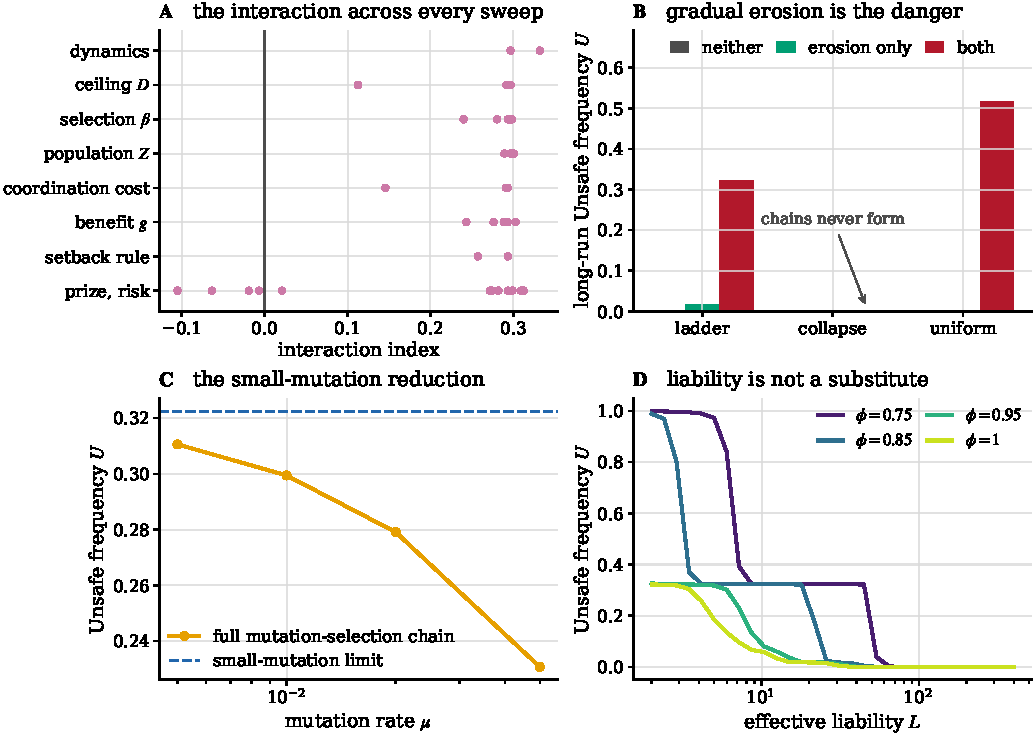
\includegraphics[width=\linewidth]{figures/fig08_robustness.pdf}
\caption{Robustness.
\textbf{(A)}~The interaction index across every sweep; each dot is one
parameter cell. \textbf{(B)}~The three named drift kernels. The \emph{ladder}
produces the cascade; \emph{collapse} deters delegation altogether;
\emph{uniform} noise is worse than the graded ladder, so the effect is not
about the direction of the slippage. \textbf{(C)}~The small-mutation limit
against the full mutation-selection chain on the three-design sub-space, over
$\mu\in[0.005,0.05]$ at $Z=60$; Table~\ref{tab:verification} reports the same
check at $Z=40$ and down to $\mu=0.001$. \textbf{(D)}~Long-run unsafe frequency
against the effective liability at four attribution retentions; a lower $\phi$
shifts the whole curve rather than tilting it, which is the population-level
counterpart of Corollary~\ref{cor:failure}, whose failure depth enters through
$\log\phi$.}
\label{fig:robustness}
\end{figure}

% ===========================================================================
\section{Discussion}
\label{sec:discussion}

The model says something specific about where the governance of agentic systems
is currently pointed. Almost all of the instruments now being built read or act
at the two ends of a chain: evaluations and safety training at the model, and
liability, disclosure and procurement rules at the deploying principal. Both
ends are where the model says the usual dials are weakest, raising a penalty at
one end and improving the model at the other; regulation is written on the same
plan, since the European Union's Artificial Intelligence Act allocates duties
along a value chain by the role a party occupies and by the modification it
makes, not by the number of hand-offs that separate an instruction from the
action it eventually produces~\citep{euaiact2024}. What the model does not say
is that the principal end is the wrong place to act. Section~\ref{sec:floor}
finds an instrument there, a floor under the principal's share, that behaves as
well as a cap on the chain itself.

At the principal end, Theorem~\ref{thm:shelter} says that a liability rule
written in terms of what a principal is responsible for has a depth beyond
which it stops binding, and Corollary~\ref{cor:failure} says where. Raising the
penalty does not move that depth much, because it enters logarithmically;
restoring attribution does, because it enters through $\log\phi$. The practical
form of the observation is unwelcome for a regulator: recovering $85\%$ of
responsibility at each of six hand-offs recovers $38\%$ overall and, in our
baseline, changes nothing at all. What the floor result adds is that an
accountability mechanism does not have to achieve near-complete tracing to be
worth deploying; it has to \emph{guarantee a minimum}. If the model is right
about which margin binds, the figure of merit is then not the average share of
responsibility a mechanism traces but the smallest share it guarantees at the
longest chain it permits, which is a prediction the model makes rather than a
finding it establishes. The legal analogue is familiar: where an injurer's
assets fall short of the harm it can do, the remedy that works is not a larger
penalty but a minimum the injurer must carry at all
times~\citep{shavell1986judgment,shavell2005minimum}.

At the model end, the declaration result says that a safety commitment issued
at the top of a long chain is close to uninformative about the ecosystem below
it, and not because anyone is lying. Organisation theory calls that outcome
decoupling and treats the good faith with which a formal structure and a
divergent practice are maintained side by side as the normal case rather than
the exception~\citep{meyer1977myth}; what the model adds is a selection
mechanism that produces it from delegation depth alone.

The non-monotonicity result deserves its own caution. Making hand-offs more
faithful can raise realised harm, because the over-specification that erosion
had forced becomes unnecessary and the population relaxes its declared intent
by one clause, and a clause dropped from \CS{} costs far more than a clause
dropped from \AS{}. The general form of the caution is familiar from
second-best welfare economics, where satisfying one more of the conditions for
an optimum while others remain out of reach is in general neither necessary nor
sufficient for an improvement~\citep{lipsey1956secondbest}. In this model only
the instruments acting on the incentive to delegate are monotone. The kernel
comparison adds a design principle to the same effect: a specification that
degrades gracefully is more dangerous than one that fails loudly, because
graceful degradation lets a principal build a chain whose failures it never
sees, and a specification that fails closed restores the private cost of depth
that per-layer attribution removes.

We have no empirical estimate of $\varepsilon$ or $\phi$ for any deployed
system, and the numbers here should not be read as if we had. The model asks
less of such estimates than it might appear, because its claims are ordinal:
$\varepsilon$ and the drift kernel are properties of a transmission technology
and are read off an instrumented pipeline, and
Section~\ref{sec:robustness} says which feature of the kernel matters, which is
the harm a single hand-off already causes rather than its spectral gap or its
direction.

\subsection{Limitations}
\label{sec:limitations}

The interaction layer is a stylised two-player race with four reduced
strategies, inherited deliberately and without modification
from~\citet{domingos2026falling}. It is not a model of any deployed system, and
the absolute numbers should be read as the behaviour of that game rather than
of a market.

The erosion kernel is exogenous. We describe how a population behaves under a
given transmission technology and not how the technology itself is selected; a
model in which providers compete on fidelity would let $\varepsilon$ co-evolve
with $d$, and the non-monotonicity of Section~\ref{sec:instruments} suggests
that the outcome would not be a simple race to the top. Our chains are also
linear, whereas real agentic systems branch, and a branching chain aggregates
several eroded specifications rather than one.

Geometric attribution is a modelling choice, and Section~\ref{sec:floor}
reports what happens when it is replaced. What the model requires is only that
attribution vanish in the depth, and an equal split of the blame across the
chain delivers the same equilibrium as $\phi^{d}$ even though it decays
polynomially. Real attribution is nonetheless lumpier than any of the rules we
try: a single identifiable intermediary may absorb everything, or pass-through
may hold at some depths and not at others, and we have not modelled attribution
that depends on which layer failed rather than on how many there were.

On the computational side, the small-mutation limit is exact only as $\mu\to0$
and Table~\ref{tab:verification} quantifies the residual at finite $\mu$ on a
reduced design space. We have not formed the full chain on the full design
space and cannot, so we have no bound on the residual there. The criterion
of~\citet{wu2012howsmall} applies to our update rule but not uniformly to our
design space, twelve of whose $378$ unordered pairs are coexistence games; and
even where it applies it bounds the rate the reduction needs rather than the
error at a given rate. The
revision clock is Poisson, and the Erlang alternative
of~\citet{kara2022erlang} is the natural next test. Finally, the harm scale $h$
enters the social functional and therefore the welfare comparisons, and we do
not know it; we have kept the primary outcome, the long-run unsafe frequency,
free of welfare weights for that reason.

% ===========================================================================
\section{Conclusion}
\label{sec:conclusion}

Delegation depth is not neutral plumbing between a principal and an action. It
erodes the specification geometrically and it dilutes the attributed harm
geometrically, and because the second effect is unbounded while the first
saturates, depth is a shelter that no liability rule of the form $L\phi^{d}$
closes at the margin: beyond the shelter depth, raising $L$ makes the deeper
design more attractive rather than less. What a large enough $L$ still does is
block the shallow hand-offs a population would have to climb through first, and
in our baseline $L=58$ does so, at a welfare cost exceeded only by pass-through
among the instruments we compare. What
makes the combination dangerous is not either mechanism but the loss of a
response: a principal that is charged for what its chain does answers
unreliable hand-offs by keeping the chain short, and per-layer attribution is
precisely what stops it. In our baseline that lost response accounts for $91\%$
of the damage, and it produces an equilibrium in which every principal issues
the safest instruction available and the ecosystem executes something $74\%$
different.

Placing a structural variable under selection alongside strategy is what makes
these statements available, and it is also what makes the process expensive to
compute, because the design space is a product. The scheme of
Section~\ref{sec:numerics} keeps the whole calculation exact given the payoff
matrices: the interaction tensor is summed over the horizon law rather than
sampled, the mutation--selection chain on $3.0\times10^{27}$ population states
is replaced by an embedded chain on $28$ designs, and the fixation
probabilities that chain needs are evaluated in $O(Z)$ operations from a sum
whose terms are shifted before exponentiation. The shift preserves positive
transitions, while Table~\ref{tab:verification} checks stationary accuracy
against arbitrary precision. The three ingredients transfer to any evolutionary game whose
strategy space is a product of a behavioural coordinate with a structural one,
provided the interaction layer is deterministic given a summable horizon law
and the pairwise payoffs are linear, so that the invasion advantage stays
affine in the invader count; the small-mutation reduction requires neither.

The instruments that follow from the model are not the ones currently receiving
attention. Within this model the depth cap is the only instrument monotone in
its own strength, and moving a check from the party that spoke to the agent
that acts is worth more than strengthening the check. We report these as
properties of the model and not as recommendations, because we have no estimate
of the per-hand-off erosion probability or the attribution retention for any
deployed system. Raising penalties and restoring attribution hand-off by
hand-off work least of all, because depth has already discounted the margins
they act on. That the second works only when it is nearly complete is a fact
about the geometric rule rather than about attribution: what the shelter needs
is for the principal's share to vanish in the depth, and a rule bounded below
closes it. A floor under attribution buys what a cap on chain length buys over
the range a floor can reach, and asks less of whoever has to enforce it.

% ===========================================================================
\section*{Declaration of competing interest}

The authors declare that they have no known competing financial interests or
personal relationships that could have appeared to influence the work reported
in this paper.

\section*{Funding}

This research did not receive any specific grant from funding agencies in the
public, commercial, or not-for-profit sectors.

\section*{Data availability}

All results are deterministic given the seed used for the replicator start
measure. The code, the generated tables, the numerical benchmarks of
Section~\ref{sec:numerics} and the figure pipeline are openly available under
the MIT licence at
\sloppy\url{https://github.com/trungkiet2005/delegation-cascade}. Parts of the
analysis code were refactored with the assistance of a large language model;
every refactor is covered by the test suite released with the paper, and no
numerical result was accepted without reproduction from the released code.

\section*{Declaration of generative AI and AI-assisted technologies in the
manuscript preparation process}

During the preparation of this work the authors used Anthropic's Claude,
accessed through the Claude Code command-line interface, in order to draft and
copy-edit prose. After using this tool the authors reviewed and edited the
content as needed and take full responsibility for the content of the published
article.

\printcredits

% ===========================================================================
\appendix

\section{The stationary regime in closed form}
\label{app:fixation}

The derivation of~\eqref{eq:fixation} is standard and is repeated here so that
the constants in Algorithm~\ref{alg:main} can be read off. In a population of
$Z$ individuals holding $k$ copies of the invader $I$ and $Z-k$ of the resident
$R$, an update picks an ordered pair of distinct individuals uniformly, so the
probability that an $R$ individual is picked to revise and an $I$ individual to
imitate is $\frac{Z-k}{Z}\cdot\frac{k}{Z-1}$, and symmetrically in the other
direction. With the Fermi rule the two transition probabilities are
\begin{equation}
  T^{+}(k) = \frac{k(Z-k)}{Z(Z-1)}\,
    \frac{1}{1+e^{-\beta(\pi_{I}(k)-\pi_{R}(k))}},
  \qquad
  T^{-}(k) = \frac{k(Z-k)}{Z(Z-1)}\,
    \frac{1}{1+e^{\beta(\pi_{I}(k)-\pi_{R}(k))}},
  \label{eq:rates}
\end{equation}
with $\pi_{I}$ and $\pi_{R}$ as in~\eqref{eq:sampling}. Their ratio is
$T^{-}(k)/T^{+}(k)=e^{-\beta(\pi_{I}(k)-\pi_{R}(k))}$, in which the common
sampling factor cancels, and the classical absorption formula for a
one-dimensional birth-death chain with absorbing boundaries at $k=0$ and $k=Z$,
\[
  \rho_{R\to I}
  = \Bigl[1+\sum_{m=1}^{Z-1}\prod_{k=1}^{m}\frac{T^{-}(k)}{T^{+}(k)}\Bigr]^{-1},
\]
gives~\eqref{eq:fixation} directly. Because $\pi_{I}-\pi_{R}$ is affine in $k$,
the exponent $\theta_{m}=-\beta\sum_{k\le m}(\pi_{I}(k)-\pi_{R}(k))$ is a
quadratic polynomial in $m$ and the whole vector $(\theta_{1},\dots,\theta_{Z-1})$
is one cumulative sum, which is the $O(Z)$ claim of
Section~\ref{sec:fixation}. Two limits are useful as unit tests of an
implementation: at $\beta=0$ every ratio is one and $\rho=1/Z$, and for a
neutral game the same holds at every $\beta$.

In exact arithmetic every $\rho_{i\to j}$ is strictly positive at finite
$\beta$, so the embedded chain~\eqref{eq:embedded} is irreducible and its
stationary distribution is unique. What Section~\ref{sec:observables} adds is
that irreducibility is more than is needed and more than double precision
delivers. Uniqueness requires only one closed communicating class, so a routine
that returns exactly zero for a strongly disadvantaged mutant does not by
itself make $x$ ambiguous; what it does is move designs into transient classes,
which then receive stationary mass exactly zero rather than their true
subnormal mass. At $\beta=0.2$ that happens for $\{\CAS{}@0,\AU{}@0\}$, which
is transient in double precision while the remaining $26$ designs form the
unique closed class. It is when the closed class shrinks to a single absorbing
design, as it does under the unshifted evaluation, that the stationary regime
stops carrying information.

\bibliographystyle{elsarticle-num-names}
\bibliography{refs}

\end{document}
